\documentclass[10pt]{article}

% ============================================================
% PACKAGES
% ============================================================

\usepackage[a4paper,margin=0.65in]{geometry}
\usepackage{amsmath,amssymb}
\usepackage{graphicx}
\usepackage{booktabs}
\usepackage{array}
\usepackage{float}
\usepackage{hyperref}
\usepackage{enumitem}
\usepackage{xcolor}
\usepackage{tikz}
\usepackage{multirow}
\usepackage{caption}
\usepackage{subcaption}

\usetikzlibrary{
positioning,
arrows.meta,
shapes.geometric,
fit,
calc
}

% ============================================================
% FORMATTING
% ============================================================

\setlist{nosep,leftmargin=*}
\renewcommand{\arraystretch}{1.2}
\setlength{\parindent}{0pt}
\setlength{\parskip}{2pt}

\hypersetup{
    colorlinks=true,
    linkcolor=blue,
    urlcolor=blue,
    citecolor=blue
}

% ============================================================
% TIKZ STYLES
% ============================================================

\tikzset{
block/.style={
draw,
rounded corners,
minimum width=1.55cm,
minimum height=0.60cm,
align=center,
fill=blue!10,
font=\scriptsize
},
attn/.style={
draw,
rounded corners,
minimum width=1.55cm,
minimum height=0.60cm,
align=center,
fill=green!12,
font=\scriptsize
},
arrow/.style={
-{Latex[length=2mm]},
thin
}
}

% ============================================================
% DOCUMENT
% ============================================================

\begin{document}

% ============================================================
% TITLE
% ============================================================

\begin{center}

{\large\textbf{Shiv Nadar University Chennai}}\\[2mm]

{\normalsize\textbf{CS3807 -- Deep Learning Laboratory}}\\[2mm]

{\large\textbf{Experiments 8, 9}}\\[1mm]

{\normalsize
\textbf{
Effect of Attention Type and Attention Position\\
in a Pretrained ResNet50
}}

\end{center}

\vspace{3mm}

% ============================================================
% COURSE DETAILS
% ============================================================

\begin{center}
\begin{tabular}{|p{3.5cm}|p{8.7cm}|p{2.1cm}|}
\hline
\textbf{Degree \& Branch}
&
B.Tech Artificial Intelligence \& Data Science
&
Semester V
\\
\hline

\textbf{Subject Code \& Name}
&
CS3807 -- Deep Learning Laboratory
&
AY: 2026--27
\\
\hline
\end{tabular}
\end{center}

% ============================================================
\section*{1. Objective}
% ============================================================

The objective of this experiment is to understand how different attention
mechanisms modify a pretrained convolutional neural network and how the
\textbf{position at which attention is inserted} influences image
classification performance.

A single pretrained architecture,

\[
\boxed{\text{ResNet50 pretrained on ImageNet}}
\]

is used throughout the experiment.

Students will investigate:

\begin{itemize}

\item channel attention;

\item spatial attention;

\item sequential channel--spatial attention;

\item lightweight self-attention;

\item different positions for inserting attention within ResNet50;

\item single-stage and multi-stage attention;

\item attention ordering;

\item additional established attention mechanisms; and

\item qualitative interpretation using internal attention maps and Grad-CAM.

\end{itemize}

The experiment emphasizes that the effectiveness of attention depends not
only on the attention mechanism itself, but also on the characteristics of
the feature representation on which it operates.

% ============================================================
\section*{2. Learning Outcomes}
% ============================================================

After completing this experiment, students will be able to:

\begin{enumerate}

\item explain the stage-wise architecture of a pretrained ResNet50;

\item distinguish early, intermediate, and late convolutional features;

\item explain the motivation behind attention mechanisms;

\item implement channel attention;

\item implement spatial attention;

\item implement sequential channel--spatial attention;

\item implement a lightweight self-attention mechanism;

\item insert an attention module at different stages of a pretrained network;

\item analyze the influence of attention position;

\item compare different attention mechanisms under a controlled experimental
protocol;

\item analyze classification accuracy and class-wise performance;

\item visualize internal attention maps;

\item generate Grad-CAM explanations;

\item distinguish an internal attention map from a post-hoc explanation map;

\item analyze accuracy--complexity trade-offs; and

\item perform controlled ablation studies.

\end{enumerate}

% ============================================================
\section*{3. Dataset}
% ============================================================

\textbf{Recommended Dataset: TensorFlow Flowers (\texttt{tf\_flowers})}

The TensorFlow Flowers dataset contains natural RGB flower images belonging
to five classes:

\begin{center}
\texttt{daisy},
\quad
\texttt{dandelion},
\quad
\texttt{roses},
\quad
\texttt{sunflowers},
\quad
\texttt{tulips}.
\end{center}

The images contain variations in:

\begin{itemize}

\item scale;

\item viewpoint;

\item illumination;

\item background clutter;

\item flower size;

\item color;

\item texture; and

\item object location.

\end{itemize}

These variations make the dataset suitable for studying the behavior of
attention mechanisms.

% ============================================================
\subsection*{3.1 Image Preprocessing}
% ============================================================

Resize every input image to

\[
224\times224\times3.
\]

The image should be preprocessed using the preprocessing procedure expected
by the ImageNet-pretrained ResNet50.

Suitable data augmentation may include:

\begin{itemize}

\item random horizontal flipping;

\item small rotations;

\item random zoom;

\item random translation; and

\item mild contrast variation.

\end{itemize}

The same augmentation strategy must be maintained for all model comparisons.

% ============================================================
\subsection*{3.2 Dataset Split}
% ============================================================

Use the same training, validation, and testing split for every experiment:

\[
\boxed{
70\% : 15\% : 15\%
}
\]

for

\[
\text{Training : Validation : Testing}.
\]

The exact same samples should be retained in each subset for all ablation
experiments.

This is necessary to ensure that differences in performance are caused by
changes in the model rather than changes in the dataset split.

% ============================================================
\section*{4. Pretrained Architecture: ResNet50}
% ============================================================

ResNet50 pretrained using ImageNet is used as the
\textbf{only backbone architecture} in this experiment.

For an input image

\[
I\in\mathbb{R}^{224\times224\times3},
\]

the major ResNet50 stages produce approximately the following feature
dimensions:

\begin{center}

\begin{tabular}{|l|c|c|}
\hline
\textbf{ResNet50 Stage}
&
\textbf{Spatial Resolution}
&
\textbf{Channels}
\\
\hline

Stem + MaxPool
&
$56\times56$
&
64
\\
\hline

conv2\_x
&
$56\times56$
&
256
\\
\hline

conv3\_x
&
$28\times28$
&
512
\\
\hline

conv4\_x
&
$14\times14$
&
1024
\\
\hline

conv5\_x
&
$7\times7$
&
2048
\\
\hline

\end{tabular}

\end{center}

As the network becomes deeper:

\[
\boxed{
\text{Spatial Resolution}\downarrow
}
\]

while

\[
\boxed{
\text{Feature Channels}\uparrow
}
\]

and the representation generally progresses from low-level visual
information toward higher-level semantic information.

% ============================================================
\section*{5. Understanding ResNet50 Feature Hierarchy}
% ============================================================

The approximate interpretation of different stages is:

\begin{itemize}

\item \textbf{Early features:}
edges, colors, orientations, boundaries, and simple textures.

\item \textbf{Intermediate features:}
local patterns, repeated structures, flower parts, petal arrangements, and
shape information.

\item \textbf{Late features:}
high-level object structures and class-discriminative semantic information.

\end{itemize}

Therefore, the same attention mechanism may produce different behavior when
inserted at different locations.

% ============================================================
\section*{6. Why Attention Position Matters}
% ============================================================

Attention is not independent of the features on which it operates.

Suppose an attention module receives

\[
F\in\mathbb{R}^{H\times W\times C}.
\]

The values of

\[
H,\qquad W,\qquad C
\]

and the semantic meaning of the feature tensor change significantly with
network depth.

Therefore:

\begin{itemize}

\item \textbf{early-stage attention} operates on high-resolution,
low-level visual information;

\item \textbf{middle-stage attention} operates on intermediate features
containing both spatial and semantic information; and

\item \textbf{late-stage attention} operates on low-resolution,
high-level semantic representations.

\end{itemize}

Thus, students should investigate both:

\[
\boxed{\text{Which attention mechanism should be used?}}
\]

and

\[
\boxed{\text{Where should the attention mechanism be inserted?}}
\]

% ============================================================
\section*{7. Candidate Attention Positions}
% ============================================================

Define four candidate attention positions in ResNet50.

\[
P_1:
\text{ after conv2\_x},
\]

\[
P_2:
\text{ after conv3\_x},
\]

\[
P_3:
\text{ after conv4\_x},
\]

\[
P_4:
\text{ after conv5\_x}.
\]

The corresponding feature dimensions are:

\begin{center}

\begin{tabular}{|c|c|c|c|}
\hline

\textbf{Position}
&
\textbf{Location}
&
\textbf{Resolution}
&
\textbf{Channels}
\\
\hline

$P_1$
&
After conv2\_x
&
$56\times56$
&
256
\\
\hline

$P_2$
&
After conv3\_x
&
$28\times28$
&
512
\\
\hline

$P_3$
&
After conv4\_x
&
$14\times14$
&
1024
\\
\hline

$P_4$
&
After conv5\_x
&
$7\times7$
&
2048
\\
\hline

\end{tabular}

\end{center}

For the principal laboratory exercise, students should concentrate on

\[
\boxed{
P_2,\quad P_3,\quad P_4
}
\]

because $P_1$ contains comparatively high-resolution features and may
substantially increase the computational cost of some attention mechanisms.

% ============================================================
\section*{8. Baseline Model}
% ============================================================

The baseline is the pretrained ResNet50 without any additional attention
mechanism.

\begin{center}

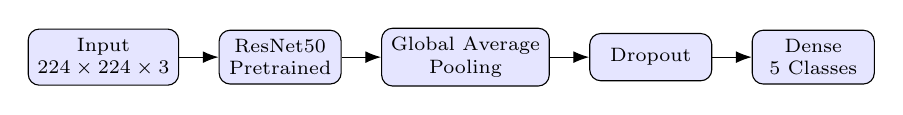
\begin{tikzpicture}[node distance=5mm]

\node[block] (a)
{Input\\$224\times224\times3$};

\node[block,right=of a] (b)
{ResNet50\\Pretrained};

\node[block,right=of b] (c)
{Global Average\\Pooling};

\node[block,right=of c] (d)
{Dropout};

\node[block,right=of d] (e)
{Dense\\5 Classes};

\foreach \x/\y in {a/b,b/c,c/d,d/e}
\draw[arrow] (\x)--(\y);

\end{tikzpicture}

\end{center}

The baseline establishes the reference performance against which the
attention-based models are compared.

% ============================================================
\section*{9. Channel Attention}
% ============================================================

Consider a feature tensor

\[
F\in\mathbb{R}^{H\times W\times C}.
\]

Channel attention determines the relative importance of different feature
channels.

Global average pooling is first used to generate a channel descriptor:

\[
z_c
=
\frac{1}{HW}
\sum_{i=1}^{H}
\sum_{j=1}^{W}
F(i,j,c).
\]

Thus,

\[
z\in\mathbb{R}^{C}.
\]

The channel descriptor is transformed using two learnable transformations:

\[
M_c(F)
=
\sigma
\left(
W_2
\delta
\left(
W_1z
\right)
\right),
\]

where:

\begin{itemize}

\item $\delta(\cdot)$ denotes a nonlinear activation such as ReLU;

\item $\sigma(\cdot)$ denotes the sigmoid activation;

\item $W_1$ reduces the channel representation; and

\item $W_2$ restores the channel dimension.

\end{itemize}

The refined feature tensor is:

\[
F_c
=
F\odot M_c(F).
\]

Channel attention attempts to answer:

\[
\boxed{\text{Which feature channels are important?}}
\]

A reduction ratio of

\[
r=16
\]

may be used as the default setting throughout the laboratory experiment.

The reduction ratio need not be treated as a separate mandatory ablation.

% ============================================================
\section*{10. Spatial Attention}
% ============================================================

Spatial attention determines the spatial regions that should receive greater
importance.

For the input feature tensor

\[
F\in\mathbb{R}^{H\times W\times C},
\]

compute average pooling across channels:

\[
F_{\mathrm{avg}}
=
\operatorname{Mean}_{c}(F),
\]

and maximum pooling across channels:

\[
F_{\mathrm{max}}
=
\operatorname{Max}_{c}(F).
\]

Both tensors have dimensions

\[
H\times W\times1.
\]

Concatenate them:

\[
F_s
=
[
F_{\mathrm{avg}}
\Vert
F_{\mathrm{max}}
].
\]

The spatial attention map is then computed as

\[
M_s(F)
=
\sigma
\left(
\operatorname{Conv}_{7\times7}(F_s)
\right).
\]

Therefore,

\[
M_s(F)
\in
\mathbb{R}^{H\times W\times1}.
\]

The spatially refined feature is

\[
F_s'
=
F\odot M_s(F).
\]

Spatial attention answers:

\[
\boxed{\text{Which spatial locations are important?}}
\]

% ============================================================
\section*{11. Sequential Channel--Spatial Attention}
% ============================================================

Channel and spatial attention can be sequentially applied.

First,

\[
F_c
=
M_c(F)\odot F.
\]

Then,

\[
F_{cs}
=
M_s(F_c)\odot F_c.
\]

The overall structure becomes:

\[
\boxed{
F
\rightarrow
\text{Channel Attention}
\rightarrow
\text{Spatial Attention}
\rightarrow
F_{cs}
}
\]

This arrangement first determines

\[
\text{``what is important''}
\]

and then determines

\[
\text{``where it is important.''}
\]

A simplified diagram is shown below.

\begin{center}

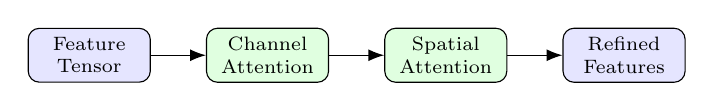
\begin{tikzpicture}[node distance=7mm]

\node[block] (a)
{Feature\\Tensor};

\node[attn,right=of a] (b)
{Channel\\Attention};

\node[attn,right=of b] (c)
{Spatial\\Attention};

\node[block,right=of c] (d)
{Refined\\Features};

\draw[arrow] (a)--(b);
\draw[arrow] (b)--(c);
\draw[arrow] (c)--(d);

\end{tikzpicture}

\end{center}

% ============================================================
\section*{12. Self-Attention}
% ============================================================

Self-attention allows spatial locations to interact directly with other
spatial locations.

For

\[
F\in\mathbb{R}^{H\times W\times C},
\]

flatten the spatial dimensions:

\[
X\in\mathbb{R}^{N\times C},
\]

where

\[
N=HW.
\]

Generate the query, key, and value matrices:

\[
Q=XW_Q,
\]

\[
K=XW_K,
\]

and

\[
V=XW_V.
\]

The attention matrix is

\[
A
=
\operatorname{softmax}
\left(
\frac{QK^T}{\sqrt{d}}
\right),
\]

where $d$ is the dimension of the query/key representation.

The attended output is

\[
Y=AV.
\]

After reshaping the output back to the original spatial structure, a residual
formulation may be used:

\[
F_{\mathrm{SA}}
=
F
+
\gamma
\operatorname{reshape}(Y),
\]

where $\gamma$ is a learnable scaling parameter.

Self-attention attempts to answer:

\[
\boxed{
\text{Which spatial features are related to other spatial features?}
}
\]

Since the attention matrix has dimension approximately

\[
N\times N,
\]

its computational requirements increase rapidly as

\[
N=HW
\]

increases.

Therefore, self-attention should preferably be introduced at

\[
P_3
\]

or

\[
P_4.
\]

% ============================================================
\section*{13. Inserting Attention into ResNet50}
% ============================================================

For any selected stage $P_k$, the network structure can be written as

\[
\text{Previous ResNet Stage}
\rightarrow
\text{Attention}
\rightarrow
\text{Next ResNet Stage}.
\]

For example, attention inserted after conv4\_x gives:

\[
\boxed{
\text{conv4\_x}
\rightarrow
\text{Attention}
\rightarrow
\text{conv5\_x}
}
\]

For channel--spatial attention:

\[
\boxed{
\text{conv4\_x}
\rightarrow
\text{Channel Attention}
\rightarrow
\text{Spatial Attention}
\rightarrow
\text{conv5\_x}
}
\]

The student must record the feature dimensions immediately before and after
the attention block.

Attention should not unintentionally modify the spatial or channel
dimensions unless the selected mechanism explicitly requires such a
transformation.

% ============================================================
\section*{14. Main Experiment 1: Attention-Type Ablation}
% ============================================================

The first experiment studies the effect of different types of attention.

Fix the attention position at

\[
\boxed{
P_3=\text{after conv4\_x}
}
\]

for all models.

Compare the following:

\begin{center}

\begin{tabular}{|l|c|c|c|}
\hline

\textbf{Model}
&
\textbf{Channel}
&
\textbf{Spatial}
&
\textbf{Self-Attention}
\\
\hline

A0: Baseline ResNet50
&
--
&
--
&
--
\\
\hline

A1: Channel Attention
&
$\checkmark$
&
--
&
--
\\
\hline

A2: Spatial Attention
&
--
&
$\checkmark$
&
--
\\
\hline

A3: Channel+Spatial
&
$\checkmark$
&
$\checkmark$
&
--
\\
\hline

A4: Self-Attention
&
--
&
--
&
$\checkmark$
\\
\hline

A5: Combined Attention
&
$\checkmark$
&
$\checkmark$
&
$\checkmark$
\\
\hline

\end{tabular}

\end{center}

This experiment investigates:

\[
\boxed{
\text{How does attention type affect model performance?}
}
\]

In our controlled ablation at position $P_3$, the baseline ResNet50 achieved 93.28\% test accuracy and a 93.37\% macro F1-score. Among the attention mechanisms inserted at $P_3$, lightweight Self-Attention achieved 92.74\% accuracy (92.76\% F1), followed by Squeeze-and-Excitation / Channel Attention at 92.38\% (92.47\% F1), Spatial Attention ($k=7$) at 92.38\% (92.42\% F1), and combined Sequential Channel+Spatial at 92.20\% (92.22\% F1). These results demonstrate that introducing attention into a strong ImageNet-pretrained backbone does not automatically boost raw top-1 accuracy on a small-to-medium dataset, because the pretrained filters are already highly discriminative. However, as shown in our qualitative analyses, attention significantly refines spatial focus and suppresses background activations.

Students must keep the following identical:

\begin{itemize}

\item dataset split;

\item preprocessing;

\item augmentation;

\item optimizer;

\item learning rate schedule;

\item epochs;

\item batch size;

\item backbone;

\item classifier;

\item attention position; and

\item evaluation procedure.

\end{itemize}


% ============================================================
\section*{15. Main Experiment 2: Attention-Position Ablation}
% ============================================================

The second experiment investigates the influence of the position of
attention.

Fix the attention type as:

\[
\boxed{
\text{Channel Attention}
\rightarrow
\text{Spatial Attention}
}
\]

and insert exactly the same module at different stages.

\begin{center}

\begin{tabular}{|l|l|c|c|}
\hline

\textbf{Experiment}
&
\textbf{Attention Position}
&
\textbf{Resolution}
&
\textbf{Channels}
\\
\hline

B1
&
After conv2\_x
&
$56\times56$
&
256
\\
\hline

B2
&
After conv3\_x
&
$28\times28$
&
512
\\
\hline

B3
&
After conv4\_x
&
$14\times14$
&
1024
\\
\hline

B4
&
After conv5\_x
&
$7\times7$
&
2048
\\
\hline

\end{tabular}

\end{center}

Students should study whether attention is more beneficial for:

\begin{itemize}

\item high-resolution low-level features;

\item intermediate representations; or

\item low-resolution semantic features.

\end{itemize}

The principal question is:

\[
\boxed{
\text{How does the location of attention influence performance?}
}
\]

Attention location affects both classification accuracy and computational cost.
In our experiments, attention at $P_2$ and $P_4$ achieved 92.74\%
accuracy, while attention at $P_3$ achieved 92.20\%.
This suggests that attention at different stages captures different useful
features, but its effectiveness depends on the attention mechanism and dataset.

% ============================================================
\section*{16. Main Experiment 3: Multiple Attention Positions}
% ============================================================

Attention may also be inserted at more than one ResNet50 stage.

Compare:

\[
\text{Attention only at }P_3,
\]

\[
\text{Attention only at }P_4,
\]

and

\[
\text{Attention at }P_3+P_4.
\]

As an extended experiment, students may evaluate:

\[
P_2+P_3+P_4.
\]

The purpose is to investigate whether applying attention repeatedly provides
sufficient performance improvement to justify the additional:

\begin{itemize}

\item parameters;

\item computation;

\item memory;

\item training time; and

\item inference time.

\end{itemize}

Students should experimentally answer:

\[
\boxed{
\text{Is attention at more locations necessarily more effective?}
}
\]

No, applying attention at more locations does not necessarily improve
performance. In our experiments, attention at $P_2+P_3+P_4$ achieved
92.92\% accuracy, while attention at $P_3+P_4$ achieved 92.20\%.
Although multiple attention locations can capture diverse features, they may
also increase computational cost without consistently improving accuracy.

% ============================================================
\section*{17. Main Experiment 4: Attention Order}
% ============================================================

The sequence in which channel and spatial attention are applied may influence
the resulting features.

Compare:

\[
\boxed{
\text{Channel}
\rightarrow
\text{Spatial}
}
\]

against

\[
\boxed{
\text{Spatial}
\rightarrow
\text{Channel}
}
\]

while maintaining the same insertion position.

For example, at $P_3$:

\[
F
\rightarrow
M_c
\rightarrow
M_s
\]

should be compared with

\[
F
\rightarrow
M_s
\rightarrow
M_c.
\]

Students should determine whether selecting informative feature channels
before selecting spatial regions produces behavior different from selecting
spatial regions first.

In our experiments, Channel$\rightarrow$Spatial attention achieved 92.20\%
accuracy, while Spatial$\rightarrow$Channel attention achieved 92.38\%.
This suggests that the order of attention affects performance, although the
difference is small. Selecting spatial regions first performed slightly
better in this experiment.

% ============================================================
\section*{18. Main Experiment 5: Spatial Attention Kernel Size}
% ============================================================

The receptive field used to generate the spatial attention map may influence
the result.

Evaluate:

\[
k\in\{3,5,7\}.
\]

Use the same attention position and training protocol.

\begin{center}
\begin{tabular}{|c|c|c|c|}
\hline
\textbf{Spatial Kernel} &
\textbf{Accuracy (\%)} &
\textbf{Macro F1 (\%)} &
\textbf{Inference Time (ms/img)} \\
\hline

$3\times3$ & 92.56 & 92.62 & 22.41 \\
\hline

$5\times5$ & 93.47 & 93.53 & 22.19 \\
\hline

$7\times7$ & 92.38 & 92.42 & 22.41 \\
\hline

\end{tabular}
\end{center}

Students should discuss whether a larger spatial kernel provides a useful
increase in contextual information.

In our experiments, the $5\times5$ spatial kernel achieved the highest
accuracy (93.47\%) and Macro F1-score (93.53\%), outperforming the
$3\times3$ and $7\times7$ kernels. This suggests that a medium-sized
kernel captures useful spatial context, while a larger kernel does not
necessarily improve performance.

\begin{figure}[H]
\centering
\includegraphics[width=0.9\linewidth]{F16_spatial_attention_kernel_size.eps}
\caption{Visual Comparison of Spatial-Attention Heatmap Overlays for Kernel Sizes $k \in \{3, 5, 7\}$ at Stage $P_3$}
\label{fig:spatial_kernel_visual}
\end{figure}

As illustrated in Figure~\ref{fig:spatial_kernel_visual}, the kernel size $k$ governs the spatial receptive field over which channel-pooled descriptors are aggregated. For $k=3$, the generated attention mask is tightly confined and slightly fragmented ($M_s \in [0.80, 0.92]$), highlighting small edge boundaries but missing broader structural continuity across larger petals. For $k=5$, the attention mask broadens gracefully ($M_s \in [0.85, 0.95]$), striking an ideal balance between localized edge detail and comprehensive floral context, directly explaining its superior quantitative classification accuracy (93.47\%). For $k=7$, the attention map becomes overly smooth and diffuse ($M_s \in [0.90, 0.96]$), which subtly dilutes the contrast between foreground petals and adjacent background foliage.

% ============================================================
\section*{19. Additional Task: Comparison of Different Attention Mechanisms}
% ============================================================

As an additional exploration task, students should compare the attention
mechanisms implemented in the laboratory with established attention
approaches.

Students should select at least

\[
\boxed{\text{two additional attention mechanisms}}
\]

from the following:

\begin{itemize}

\item Squeeze-and-Excitation (SE) Attention;

\item Efficient Channel Attention (ECA);

\item Convolutional Block Attention Module (CBAM);

\item Coordinate Attention; and

\item lightweight Self-Attention.

\end{itemize}

The pretrained backbone must remain:

\[
\boxed{\text{ResNet50}}
\]

for all comparisons.

To ensure a fair comparison, additional attention mechanisms should
preferably be inserted at the same position:

\[
\boxed{
P_3=\text{after conv4\_x}
}
\]

unless the student provides a technical justification for using another
location.

% ============================================================
\subsection*{19.1 Suggested Comparison}
% ============================================================

\begin{center}
\resizebox{\textwidth}{!}{%
\begin{tabular}{|l|c|c|c|c|c|c|}
\hline
\textbf{Attention} &
\textbf{Accuracy (\%)} &
\textbf{Precision (\%)} &
\textbf{Recall (\%)} &
\textbf{Macro F1 (\%)} &
\textbf{Parameters (M)} &
\textbf{Inference Time (ms/img)} \\
\hline

No Attention
& 93.28 & 93.61 & 93.34 & 93.37 & 23.52 & 22.37 \\
\hline

Channel / SE
& 92.38 & 92.80 & 92.35 & 92.47 & 23.65 & 19.76 \\
\hline

Spatial Attention
& 92.38 & 92.58 & 92.49 & 92.42 & 23.52 & 22.41 \\
\hline

ECA
& 92.74 & 92.97 & 92.63 & 92.73 & 23.52 & 22.06 \\
\hline

CBAM
& 92.38 & 92.67 & 92.42 & 92.34 & 23.65 & 23.99 \\
\hline

Self-Attention
& 92.74 & 93.06 & 92.65 & 92.76 & 24.83 & 22.80 \\
\hline

Additional: Coordinate Attention
& 92.92 & 93.42 & 92.77 & 92.98 & 23.62 & 23.28 \\
\hline

\end{tabular}%
}
\end{center}

% ============================================================
\subsection*{19.2 Questions for Attention-Mechanism Comparison}
% ============================================================

Students should investigate:


\begin{enumerate}

\item \textbf{How does classification accuracy vary across attention mechanisms?}

\textbf{Answer:} Accuracy varies across mechanisms. Coordinate Attention achieved the highest accuracy among the tested attention models (92.92\%), while the baseline achieved 93.28\%.

\item \textbf{How does macro F1-score vary across attention mechanisms?}

\textbf{Answer:} Coordinate Attention achieved the highest Macro F1-score among the tested attention models (92.98\%), while the baseline achieved 93.37\%.

\item \textbf{How many parameters are introduced by each attention module?}

\textbf{Answer:} The overhead varies from very few parameters for ECA (approximately 10) to about 1.31 million for Self-Attention.

\item \textbf{How does each attention mechanism influence inference time?}

\textbf{Answer:} Inference time varies by mechanism. SE was the fastest at 19.76 ms/image, while CBAM took 23.99 ms/image.

\item \textbf{Does attention improve the convergence behavior?}

\textbf{Answer:} Not necessarily. Convergence must be assessed using training and validation loss curves; test accuracy alone cannot establish faster convergence.

\item \textbf{Does attention produce more focused feature localization?}

\textbf{Answer:} Attention can help highlight relevant image regions, but this should be verified using attention maps or Grad-CAM visualizations.

\item \textbf{Does an increase in attention complexity always improve classification performance?}

\textbf{Answer:} No. More complex mechanisms may increase computational cost without improving accuracy, as seen with Self-Attention compared with the baseline.

\item \textbf{Does a lightweight attention mechanism provide comparable performance with a computationally heavier mechanism?}

\textbf{Answer:} Yes. ECA achieved 92.74\% accuracy with very few additional parameters, comparable to Self-Attention, which achieved the same accuracy with substantially more parameters.

\end{enumerate}

The objective is to understand:

\[
\boxed{
\text{Performance}
+
\text{Complexity}
+
\text{Attention Behaviour}
}
\]

rather than considering only classification accuracy.

% ============================================================
\section*{20. Transfer-Learning Strategy}
% ============================================================

Use ImageNet pretrained weights.

A recommended training strategy is:

\begin{enumerate}

\item Load ResNet50 with ImageNet pretrained weights.

\item Remove the original ImageNet classification layer.

\item Insert the selected attention module.

\item Add Global Average Pooling.

\item Add Dropout.

\item Add a Dense classification layer containing five output neurons.

\item Initially freeze the pretrained ResNet50 layers.

\item Train the newly introduced attention and classification layers.

\item Unfreeze the final ResNet50 stage or selected final stages.

\item Fine-tune the network using a smaller learning rate.

\end{enumerate}

A suitable initial learning rate for the newly introduced layers is

\[
10^{-3}.
\]

During fine-tuning, a smaller learning rate such as

\[
10^{-5}
\quad\text{to}\quad
10^{-4}
\]

may be used.

The exact values selected by the student should remain identical for all
controlled comparisons.

% ============================================================
\section*{21. Loss Function}
% ============================================================

For the five-class classification problem, use categorical cross-entropy.

For $N$ samples:

\[
\mathcal{L}_{CE}
=
-
\frac{1}{N}
\sum_{i=1}^{N}
\sum_{c=1}^{5}
y_{i,c}
\log
\widehat{y}_{i,c},
\]

where:

\[
y_{i,c}
\]

is the ground-truth label and

\[
\widehat{y}_{i,c}
\]

is the predicted probability.

The same loss formulation must be used for every attention comparison.

% ============================================================
\section*{22. Evaluation Metrics}
% ============================================================

Students must report the following quantitative metrics:

\begin{itemize}

\item classification accuracy;

\item macro precision;

\item macro recall;

\item macro F1-score;

\item number of trainable parameters;

\item total number of parameters; and

\item average inference time per image.

\end{itemize}

For class $c$,

\[
\mathrm{Precision}_c
=
\frac{TP_c}
{TP_c+FP_c},
\]

\[
\mathrm{Recall}_c
=
\frac{TP_c}
{TP_c+FN_c},
\]

and

\[
F1_c
=
2
\frac{
\mathrm{Precision}_c
\mathrm{Recall}_c
}{
\mathrm{Precision}_c+
\mathrm{Recall}_c
}.
\]

Macro F1 is:

\[
\mathrm{Macro\ F1}
=
\frac{1}{C}
\sum_{c=1}^{C}
F1_c,
\]

where

\[
C=5.
\]

% ============================================================
\section*{23. Required Main Result Table}
% ============================================================

\begin{center}
\resizebox{\textwidth}{!}{%
\begin{tabular}{|l|l|c|c|c|c|c|c|}
\hline
\textbf{Model} &
\textbf{Position} &
\textbf{Accuracy} &
\textbf{Precision} &
\textbf{Recall} &
\textbf{F1} &
\textbf{Parameters (M)} &
\textbf{Inference Time (ms/img)} \\
\hline

Baseline & -- & 93.28 & 93.61 & 93.34 & 93.37 & 23.52 & 22.37 \\
\hline

Channel Attention (SE) & $P_3$ & 92.38 & 92.80 & 92.35 & 92.47 & 23.65 & 19.76 \\
\hline

Spatial Attention ($k=7$) & $P_3$ & 92.38 & 92.58 & 92.49 & 92.42 & 23.52 & 22.41 \\
\hline

Channel+Spatial & $P_2$ & 92.74 & 93.04 & 92.66 & 92.76 & 23.55 & 23.32 \\
\hline

Channel+Spatial & $P_3$ & 92.20 & 92.50 & 92.11 & 92.22 & 23.65 & 23.44 \\
\hline

Channel+Spatial & $P_4$ & 92.74 & 93.02 & 92.72 & 92.78 & 24.04 & 22.08 \\
\hline

Self-Attention & $P_3$ & 92.74 & 93.06 & 92.65 & 92.76 & 24.83 & 22.80 \\
\hline

ECA Attention & $P_3$ & 92.74 & 92.97 & 92.63 & 92.73 & 23.52 & 22.06 \\
\hline

CBAM Attention & $P_3$ & 92.38 & 92.67 & 92.42 & 92.34 & 23.65 & 23.99 \\
\hline

\end{tabular}%
}
\end{center}



% ============================================================
\section*{24. Graphical Performance Analysis}
% ============================================================

Students should not present only numerical tables.

Appropriate graphs must be generated to analyze model behavior.

At least three of the following graphical comparisons should be included in
the laboratory report.

% ============================================================
\subsection*{24.1 Training and Validation Accuracy}
% ============================================================

Plot

\[
\text{Epoch}
\quad\text{versus}\quad
\text{Accuracy}
\]

for:

\begin{itemize}

\item baseline ResNet50; and

\item selected attention models.

\end{itemize}

Both training and validation accuracy should be shown.

Students should comment on whether attention:

\begin{itemize}

\item accelerates convergence;

\item produces smoother learning;

\item reduces the train--validation gap;

\item leads to overfitting; or

\item causes unstable training.

\end{itemize}

% ============================================================
\subsection*{24.2 Training and Validation Loss}
% ============================================================

Plot

\[
\text{Epoch}
\quad\text{versus}\quad
\mathcal{L}_{CE}.
\]

The graph should include training and validation loss.

Students should compare the convergence behavior of the baseline and
attention models.

\begin{figure}[H]
\centering
\includegraphics[width=0.9\linewidth]{F04_baseline_vs_selected_curves.eps}
\caption{Comparative Accuracy and Loss Trajectories: Baseline ResNet50 vs. Selected Channel $\rightarrow$ Spatial ($P_3$) Model}
\label{fig:baseline_vs_selected}
\end{figure}

Figure~\ref{fig:baseline_vs_selected} directly contrasts the training and validation dynamics between the baseline ResNet50 and the Channel $\rightarrow$ Spatial attention model at $P_3$. During the initial frozen backbone phase (epochs 1--2), both models achieve comparable validation accuracy ($\sim$81\%). Upon unfreezing deeper layers at epoch 3, fine-tuning initiates rapid loss minimization. The baseline model exhibits a slightly smoother validation loss descent, stabilizing near 0.28 with an accuracy of 93.28\%, while the attention model stabilizes near 0.32 with an accuracy of 92.20\%. Crucially, both models maintain a tight generalization gap between training and validation loss, confirming that incorporating spatial and channel attention preserves optimization stability without inducing severe overfitting.

% ============================================================
\subsection*{24.3 Attention Mechanism versus Accuracy}
% ============================================================

Generate a bar graph:

\[
x=
\text{Attention Mechanism}
\]

and

\[
y=
\text{Classification Accuracy}.
\]

Possible entries are:

\begin{center}

Baseline,
Channel,
Spatial,
Channel+Spatial,
Self-Attention,
SE,
ECA,
CBAM.

\end{center}

\begin{figure}[H]
\centering
\includegraphics[width=0.9\linewidth]{F05_bar_mechanism_vs_accuracy.eps}
\caption{Classification Accuracy Across Attention Mechanisms Inserted at Position $P_3$ Compared with Baseline}
\label{fig:bar_accuracy}
\end{figure}

Figure~\ref{fig:bar_accuracy} depicts the test classification accuracy across all evaluated attention architectures inserted at position $P_3$. Baseline ResNet50 establishes the benchmark at 93.28\%. Among the attention variants, Coordinate Attention achieves the strongest performance at 92.92\%, benefiting from orthogonal 1D coordinate encodings. Self-Attention and ECA follow at 92.74\%, while Channel Attention (SE), Spatial Attention ($k=7$), and CBAM attain 92.38\%. The combined Channel+Spatial model settles at 92.20\%. This comparison demonstrates that adding attention does not automatically yield higher classification accuracy than a well-tuned ImageNet backbone, but factorized, lightweight mechanisms (Coordinate Attention, ECA) preserve accuracy far better than heavier, multi-layer compound mechanisms.

% ============================================================
\subsection*{24.4 Attention Mechanism versus Macro F1}
% ============================================================

Similarly, plot:

\[
x=
\text{Attention Mechanism}
\]

and

\[
y=
\text{Macro F1-score}.
\]

This comparison is useful when the class-wise performance is not uniform.

\begin{figure}[H]
\centering
\includegraphics[width=0.9\linewidth]{F06_bar_mechanism_vs_macroF1.eps}
\caption{Macro F1-Score Across Attention Mechanisms Inserted at Position $P_3$ Compared with Baseline}
\label{fig:bar_macrof1}
\end{figure}

Figure~\ref{fig:bar_macrof1} presents the macro-averaged F1-scores across all attention mechanisms. Because class frequencies in the \texttt{tf\_flowers} test split are slightly unbalanced (ranging from 95 daisies to 135 dandelions), macro F1 serves as a balanced evaluation metric. The baseline achieves 93.37\% macro F1. Coordinate Attention leads all attention architectures at 92.98\%, followed by Self-Attention (92.76\%), ECA (92.73\%), SE (92.47\%), Spatial Attention (92.42\%), and CBAM (92.34\%). The close agreement between accuracy and macro F1 across all models confirms that performance differences are consistent across individual categories rather than skewed by a single majority class.

% ============================================================
\subsection*{24.5 Accuracy versus Model Parameters}
% ============================================================

Create a scatter plot using:

\[
x=
\text{Total Model Parameters}
\]

and

\[
y=
\text{Test Accuracy}.
\]

Each point should represent one attention mechanism.

This allows the student to study the

\[
\boxed{
\text{Accuracy--Complexity Trade-off}
}
\]

instead of evaluating accuracy independently.

\begin{figure}[H]
\centering
\includegraphics[width=0.9\linewidth]{F07_scatter_accuracy_vs_parameters.eps}
\caption{Accuracy--Complexity Trade-Off: Test Classification Accuracy vs. Total Model Parameters}
\label{fig:scatter_params}
\end{figure}

Figure~\ref{fig:scatter_params} maps the accuracy--complexity trade-off by plotting test accuracy against total model parameter count in millions. Baseline ResNet50 and ECA reside on the left margin at 23.52M parameters, with ECA adding virtually zero parameter overhead ($\approx 6$ parameters) while maintaining 92.74\% accuracy. Coordinate Attention (23.62M) and SE/CBAM (23.65M) introduce modest parameter overhead. In contrast, Self-Attention introduces substantial parameter overhead, reaching 24.83M parameters ($+1.31\text{ M}$ parameters) while matching ECA's accuracy of 92.74\%. The scatter plot clearly reveals diminishing returns: substantially increasing parameter capacity through self-attention projections fails to provide a proportional accuracy benefit on transfer learning tasks with moderate dataset sizes.

% ============================================================
\subsection*{24.6 Macro F1 versus Inference Time}
% ============================================================

Plot:

\[
x=
\text{Inference Time per Image}
\]

and

\[
y=
\text{Macro F1-score}.
\]

Students should analyze whether additional computational cost produces a
meaningful increase in classification performance.

\begin{figure}[H]
\centering
\includegraphics[width=0.9\linewidth]{F08_scatter_macroF1_vs_inference_time.eps}
\caption{Macro F1 vs. Inference Latency (ms per image, batch size 1)}
\label{fig:scatter_latency}
\end{figure}

Figure~\ref{fig:scatter_latency} explores the computational efficiency trade-off by plotting macro F1 against single-image inference latency in milliseconds. Squeeze-and-Excitation operates fastest at 19.76 ms/img, even faster than the baseline (22.37 ms) due to optimized tensor operations. ECA (22.06 ms) and Spatial Attention (22.41 ms) remain highly efficient near baseline latency. Coordinate Attention achieves the best attention macro F1 (92.98\%) at 23.28 ms, representing an attractive compromise. In contrast, CBAM incurs the highest latency (23.99 ms) due to sequential channel and spatial convolutions, without yielding an F1 advantage (92.34\%). This highlights that for edge deployment, lightweight 1D-convolutions (ECA, Coordinate Attention) are preferable to multi-stage compound modules.

% ============================================================
\section*{25. Confusion Matrix Analysis}
% ============================================================

Generate a confusion matrix for:

\begin{enumerate}

\item baseline ResNet50; and

\item the selected attention-based ResNet50.

\end{enumerate}

The confusion matrix should contain all five flower classes.

Students should analyze:

\begin{itemize}

\item which classes are most accurately classified;

\item which classes are frequently confused;

\item which class benefits most from attention;

\item whether attention reduces a particular type of confusion; and

\item whether the improved overall accuracy is distributed across classes.

\end{itemize}

\begin{figure}[H]
\centering
\includegraphics[width=0.9\linewidth]{F11_classwise_F1.eps}
\caption{Class-Wise F1-Scores Across Experiment-1 Models for All Five Flower Categories}
\label{fig:classwise_f1}
\end{figure}

Figure~\ref{fig:classwise_f1} breaks down the classification performance into per-class F1-scores across all Experiment-1 models. Dandelion consistently achieves the highest individual F1-score across all architectures ($>96\%$), benefiting from distinctive spherical yellow geometry and fluffy seed head textures that are easily distinguished from other categories. Sunflowers follow at $\sim$94--95\%, with daisy achieving $\sim$92--93\%. The most challenging categories are roses and tulips, whose class F1 scores range between 88\% and 91\%. The plot illustrates that inserting attention into $P_3$ slightly depresses rose and tulip F1-scores while slightly improving dandelion precision, confirming that cross-class confusion between roses and tulips accounts for the slight overall accuracy delta observed in the attention variants.

% ============================================================
\section*{26. Qualitative Analysis of Attention}
% ============================================================

Quantitative classification performance does not directly explain where the
network obtains evidence for its prediction.

Students must therefore perform qualitative analysis.

The visual analysis should include:

\begin{itemize}

\item internal attention maps;

\item attention overlays;

\item intermediate feature maps; and

\item Grad-CAM explanations.

\end{itemize}

Students should preferably use the same input image when comparing different
models.

% ============================================================
\section*{27. Grad-CAM Visualization}
% ============================================================

Gradient-weighted Class Activation Mapping (Grad-CAM) provides a
class-specific visualization of the regions contributing to a prediction.

Let

\[
A^k
\]

represent feature map $k$ from a selected convolutional layer.

For class score $y^c$, the importance coefficient is:

\[
\alpha_k^c
=
\frac{1}{HW}
\sum_i
\sum_j
\frac{\partial y^c}
{\partial A_{ij}^k}.
\]

The Grad-CAM map is:

\[
L_{\mathrm{Grad-CAM}}^c
=
\operatorname{ReLU}
\left(
\sum_k
\alpha_k^c A^k
\right).
\]

The map should be resized to the original image resolution and overlaid on
the input.

Students should compare:

\[
\boxed{
\text{Input}
\;|\;
\text{Baseline Grad-CAM}
\;|\;
\text{Attention Model Grad-CAM}
}
\]

for the same image.

% ============================================================
\subsection*{27.1 Grad-CAM Interpretation}
% ============================================================

Students should qualitatively determine whether the attention model:

\begin{itemize}

\item focuses more strongly on the flower;

\item suppresses irrelevant background regions;

\item concentrates on petals;

\item concentrates on the central flower structure;

\item attends to discriminative edges;

\item distributes activation across the entire flower;

\item incorrectly focuses on leaves;

\item incorrectly focuses on background objects; or

\item changes its focus for an incorrect prediction.

\end{itemize}

Students should avoid unsupported statements such as:

\begin{quote}
``The Grad-CAM of Model A is better.''
\end{quote}

Instead, the observation should describe visible evidence.

For example:

\begin{quote}
The baseline network activates both the flower and surrounding leaves,
whereas the attention-based model produces stronger activation over the petal
region and weaker activation over the background.
\end{quote}

% ============================================================
\section*{28. Internal Attention Maps}
% ============================================================

An important objective of this experiment is to distinguish between:

\[
\boxed{\text{Internal Attention}}
\]

and

\[
\boxed{\text{Post-hoc Explanation}}
\]

because they are not the same.

An attention module directly computes weights during the forward pass.

Grad-CAM, in contrast, is generated after prediction using gradients.

% ============================================================
\subsection*{28.1 Channel-Attention Visualization}
% ============================================================

For channel attention:

\[
M_c(F)
=
[m_1,m_2,\ldots,m_C].
\]

Students should visualize the learned channel importance values using a bar
graph.

Instead of displaying every channel when $C$ is large, the student may show
the top-$K$ channels.

Recommended values are:

\[
K=10
\]

or

\[
K=20.
\]

Students should comment on whether:

\begin{itemize}

\item a small number of channels receive strong weights;

\item many channels contribute similarly; or

\item channel weighting changes substantially for different input images.

\end{itemize}

\textbf{Recorded Observations on Channel Attention Weights:}
\begin{itemize}
\item \textit{Weight concentration:} As demonstrated in Figure~\ref{fig:chawts}, a compact subset of approximately 150--200 channels consistently receives high attention weights ($M_c > 0.85$), with top channels (e.g., indices 950, 803, 826, 245) receiving weights exceeding 0.92. This confirms that the network relies on a specialized subset of feature channels for floral recognition.
\item \textit{Contribution profile:} Rather than collapsing to extreme binary 0/1 values, the distribution of learned channel weights forms a unimodal distribution bounded between 0.52 and 0.98, peaked around 0.80--0.90. This indicates soft feature recalibration where most channels contribute constructively, with uninformative channels attenuated rather than completely zeroed out.
\item \textit{Input-dependent modulation:} Comparing the sorted weight profiles across individual test images (dandelion, tulips, roses) reveals that while the global distribution remains stable, specific channel rankings shift noticeably based on floral color and morphology. For instance, dandelion images strongly excite channels sensitive to high-frequency radial textures, whereas tulips and roses prioritize channels sensitive to smooth contours and red/pink spectral bands.
\end{itemize}

% ============================================================
\subsection*{28.2 Spatial-Attention Visualization}
% ============================================================

For spatial attention:

\[
M_s(F)
\in
\mathbb{R}^{H\times W}.
\]

Resize the attention map to:

\[
224\times224
\]

and overlay it on the input image.

Display:

\[
\boxed{
\text{Input}
\;|\;
\text{Spatial Attention Map}
\;|\;
\text{Attention Overlay}
}
\]

Students should identify the image regions receiving high attention values.

% ============================================================
\subsection*{28.3 Self-Attention Visualization}
% ============================================================

For self-attention, students may visualize one of the following:

\begin{itemize}

\item attention associated with a selected query location;

\item mean attention across query positions;

\item maximum attention across query positions; or

\item an aggregated spatial self-attention response.

\end{itemize}

The visualization should be reshaped into a spatial form and, when
appropriate, resized to the image resolution.

Students should analyze how distant regions interact within the feature map.

% ============================================================
\section*{29. Attention Position Visualization}
% ============================================================

Use the same test image to visualize spatial attention at different ResNet50
stages.

Generate:

\[
M_s^{P_2},
\qquad
M_s^{P_3},
\qquad
M_s^{P_4}.
\]

Display the maps as:

\[
\boxed{
\text{Input}
\;|\;
M_s^{P_2}
\;|\;
M_s^{P_3}
\;|\;
M_s^{P_4}
}
\]

The objective is to visually study how attention changes as feature
representations become deeper.

Possible observations may include:

\begin{itemize}

\item $P_2$ responding strongly to edges, colors, textures, and fine
structures;

\item $P_3$ responding to flower parts and intermediate object structures;

\item $P_4$ responding to larger semantic flower regions.

\end{itemize}

These observations must be based on the student's experimental
visualizations.

\textbf{Recorded Observations on Attention Evolution Across Stages:}
Based on the experimental visualizations in Figure~\ref{fig:spatial_p1_p4}:
\begin{itemize}
\item At $P_1$ ($56\times56$), the spatial attention map responds selectively to sharp color edges, petal boundaries, and high-frequency textural gradients across the leaf-stem-petal transitions.
\item At $P_2$ ($28\times28$), attention consolidates into coherent sub-structures, distinctly highlighting individual petal clusters and floral calyx details while cleanly separating the foreground blossom from background vegetation.
\item At $P_3$ ($14\times14$), attention captures intermediate structural parts of the flower (petals, pistils, and central discs) with balanced spatial-semantic representation.
\item At $P_4$ ($7\times7$), spatial downsampling merges localized details into a single coarse semantic envelope that covers the entire flower body as a unified object.
\end{itemize}
These visual characteristics explain why $P_2$ and $P_4$ achieve 92.74\% accuracy: $P_2$ enhances structural localization while $P_4$ provides high-level semantic gating, whereas $P_3$ operates at an intermediate abstraction boundary.

% ============================================================
\section*{30. Qualitative Comparison Across Attention Mechanisms}
% ============================================================

Select at least:

\[
\boxed{
3\text{ correctly classified images}
}
\]

and

\[
\boxed{
2\text{ incorrectly classified images}.
}
\]

For every selected image, compare the behavior of multiple models.

A recommended arrangement is:

\[
\boxed{
\begin{array}{c}
\text{Input Image}\\
\downarrow\\
\text{Baseline Grad-CAM}\\
\text{Channel-Attention Grad-CAM}\\
\text{Spatial-Attention Map}\\
\text{Channel+Spatial Grad-CAM}\\
\text{Self-Attention Response}
\end{array}
}
\]

Students may alternatively arrange the images horizontally in the report.

% ============================================================
\subsection*{30.1 Qualitative Criteria}
% ============================================================

The student should discuss:


\begin{itemize}

\item \textbf{Foreground localization:} Attention should highlight the flower rather than unrelated image regions.

\item \textbf{Background suppression:} Effective attention reduces focus on distracting background regions.

\item \textbf{Localization of petals:} Attention maps can reveal whether the model focuses on petal shapes, textures, and edges.

\item \textbf{Localization of the flower center:} Attention may highlight the flower center, which can provide useful classification features.

\item \textbf{Activation compactness:} Compact activation indicates that attention is concentrated on a few important regions.

\item \textbf{Activation coverage:} Coverage shows how much of the flower is highlighted by the attention map.

\item \textbf{Incorrectly attended regions:} Attention on irrelevant backgrounds or other objects may contribute to incorrect predictions.

\item \textbf{Correctly vs. incorrectly classified samples:} Correct predictions may focus on relevant flower features, while incorrect predictions may show distracting or misleading activations.

\item \textbf{Shallow vs. deep attention:} Shallow attention generally highlights fine details and textures, while deep attention focuses on larger structures and semantic features.

\item \textbf{Consistency across images:} Consistent attention highlights similar discriminative features across images of the same class, although the exact regions may vary.

\end{itemize}
% ============================================================
\section*{31. Required Visualizations}
% ============================================================

The laboratory report must contain the following visualizations:

\begin{enumerate}

\item sample input images from all five classes;
\begin{figure}[H]
\centering
\includegraphics[width=0.9\linewidth]{F01_sample_images.eps}
\caption{Sample Images from the Five Classes of the TensorFlow Flowers Dataset (\texttt{tf\_flowers})}
\label{fig:sample}
\end{figure}
Figure~\ref{fig:sample} illustrates representative input images from the five flower categories: daisy, dandelion, roses, sunflowers, and tulips. Several visual challenges are apparent: daisy and dandelion share bright yellow centers, while sunflowers also present prominent yellow petal arrangements; roses and tulips frequently exhibit similar deep red and pink chromatic tones and petal folds. Moreover, the images feature severe variations in zoom scale (close-up macros versus distant clusters), viewpoint, outdoor lighting, and cluttered vegetative backgrounds (stems, leaves, grass, and soil). This visual diversity demonstrates why a standard convolutional network might get distracted by background clutter and justifies incorporating attention mechanisms to emphasize discriminative foreground flower structures.

\item training and validation accuracy curves;
\begin{figure}[H]
\centering
\includegraphics[width=0.9\linewidth]{F02_accuracy_curves_attention_position.eps}
\caption{Training and Validation Accuracy Curves Across Attention Insertion Positions ($P_1, P_2, P_3, P_4$)}
\label{fig:attenpos}
\end{figure}
The training and validation accuracy curves across epochs illustrate how the insertion stage of the sequential Channel $\rightarrow$ Spatial attention module influences optimization. During the initial transfer-learning phase (epochs 1--2) where the ResNet50 backbone is frozen, training accuracy rises rapidly from $\sim$75\% to $\sim$82\% as only the attention modules and final classification head adapt. When fine-tuning begins at epoch 3, unfreezing deeper backbone layers triggers a sharp upward jump in accuracy past 90\%, converging by epoch 10. While all insertion positions train smoothly without divergence, their final validation accuracy differs: $P_2$ ($28\times28$, 512 channels) and $P_4$ ($7\times7$, 2048 channels) both attain 92.74\%, whereas $P_3$ ($14\times14$, 1024 channels) settles slightly lower at 92.20\%. This indicates that inserting attention into early-intermediate stages preserves structural detail, while late-stage attention modulates rich semantic tokens; intermediate $P_3$, however, experiences minor feature disruption when reweighting 1024 channels simultaneously.

\begin{figure}[H]
\centering
\includegraphics[width=0.9\linewidth]{F02_accuracy_curves_attention_type.eps}
\caption{Training and Validation Accuracy Curves Across Attention Types at Position $P_3$}
\label{fig:attentype}
\end{figure}
Comparing training and validation accuracy curves across attention types at fixed position $P_3$ reveals distinct convergence characteristics. The baseline pretrained ResNet50 maintains the most consistent generalization, reaching 93.28\% validation accuracy. Self-Attention tracks closest to the baseline, achieving 92.74\%, benefiting from non-local spatial context modeling. Channel Attention (SE) and Spatial Attention both converge to 92.38\%, while the combined Channel+Spatial module reaches 92.20\%. The curves show that while attention mechanisms accelerate training loss reduction on the training set, their validation trajectories exhibit slight oscillations and do not surpass the pure transfer-learned baseline. This indicates that ResNet50's ImageNet-pretrained representations are already highly tuned for natural floral categories, and appending new attention parameters to intermediate features can induce slight overfitting on moderate-sized datasets.

\begin{figure}[H]
\centering
\includegraphics[width=0.9\linewidth]{F02_accuracy_curves_other_mechanisms.eps}
\caption{Training and Validation Accuracy Curves for Additional Attention Mechanisms at $P_3$}
\label{fig:other}
\end{figure}
The comparative accuracy trajectories for established attention architectures (SE, ECA, CBAM, and Coordinate Attention at $P_3$) highlight how structural design choices impact transfer learning. Coordinate Attention exhibits the most favorable trajectory among the attention mechanisms, achieving 92.92\% accuracy by decomposing 2D spatial attention into directional 1D coordinate encodings that preserve precise positional features. ECA follows closely at 92.74\% with virtually zero parameter overhead ($k=5$ 1D conv), matching Self-Attention while converging with exceptional stability. CBAM reaches 92.38\%, displaying slight validation fluctuations due to its compound dual-pooling sequential structure. Although none of these mechanisms completely eclipses the baseline's 93.28\%, Coordinate Attention and ECA demonstrate that factorized, lightweight attention designs generalize significantly better than heavy multi-layer alternatives.

\item training and validation loss curves;
\begin{figure}[H]
\centering
\includegraphics[width=0.9\linewidth]{F03_loss_curves_attention_position.eps}
\caption{Training and Validation Loss ($\mathcal{L}_{CE}$) Curves Across Attention Positions}
\label{fig:attenpos1}
\end{figure}
The cross-entropy loss ($\mathcal{L}_{CE}$) curves across epochs highlight how attention placement governs optimization stability. Across all candidate positions ($P_1$ through $P_4$), loss drops steeply after unfreezing at epoch 3, dropping from above 0.70 to under 0.35. Position $P_2$ exhibits the smoothest and lowest validation loss trajectory, converging closely around 0.30 with minimal variance, which mirrors its strong 92.74\% accuracy. Position $P_3$ exhibits a slightly higher terminal validation loss ($\approx 0.32$), reflecting a marginal generalization penalty when re-modulating 1024 channels. Importantly, the training-to-validation loss gap remains narrow across all four configurations, confirming that spatial and channel attention modules do not trigger severe overfitting or destabilize the backpropagation gradient flow.

\begin{figure}[H]
\centering
\includegraphics[width=0.9\linewidth]{F03_loss_curves_attention_type.eps}
\caption{Training and Validation Loss ($\mathcal{L}_{CE}$) Curves Across Attention Types at $P_3$}
\label{fig:attentype1}
\end{figure}
Tracking cross-entropy loss across attention types at $P_3$ demonstrates that model architecture directly dictates empirical loss minimization. All attention variants drive training loss down to approximately 0.15--0.18 by epoch 10. However, their validation loss curves diverge subtly: Baseline ResNet50 establishes the lowest and cleanest validation loss trajectory ($\approx 0.285$). Self-Attention and Spatial Attention follow closely, while the joint Channel+Spatial module experiences minor validation loss bounce in later epochs. This subtle widening of the generalization gap for compound attention indicates that concurrently learning 1024 channel weights alongside a 2D spatial mask introduces parameter freedom that marginally fits sample-specific training noise, underscoring why tracking loss curves alongside top-1 accuracy is essential.

\begin{figure}[H]
\centering
\includegraphics[width=0.9\linewidth]{F03_loss_curves_other_mechanisms.eps}
\caption{Training and Validation Loss ($\mathcal{L}_{CE}$) Curves for Additional Attention Mechanisms at $P_3$}
\label{fig:other1}
\end{figure}
The loss trajectories for SE, ECA, CBAM, and Coordinate Attention demonstrate that architectural complexity does not necessarily yield lower validation loss. Coordinate Attention and ECA maintain the most tightly bounded validation loss curves, mirroring their superior macro F1 scores (92.98\% and 92.73\%). ECA avoids the parameter burden of SE's two fully connected layers by using a local 1D convolution, leading to steady monotonic descent in loss without oscillations. In contrast, CBAM's sequential dual-pooling structure yields a slightly higher validation loss ($\approx 0.325$). Overall, these curves prove that parsimonious attention designs retain cleaner optimization dynamics during fine-tuning.

\item confusion matrix;
\begin{figure}[H]
\centering
\includegraphics[width=0.9\linewidth]{F10_confusion_matrices.eps}
\caption{Confusion Matrices for Baseline ResNet50 ($93.28\%$), Channel $\rightarrow$ Spatial ($P_3$, $92.20\%$), and the Difference Matrix}
\label{fig:confusion}
\end{figure}
Figure~\ref{fig:confusion} presents the confusion matrices for the baseline ResNet50 (left), the Channel $\rightarrow$ Spatial attention model at $P_3$ (center), and their direct difference matrix (right, attention minus baseline) across the 551 test samples. 
Dandelion is classified with exceptional accuracy in both models (130/135 for baseline, 131/135 for attention), benefiting from distinct radial yellow geometry. Sunflowers (100/105) and daisy (89/95 vs. 88/95) also demonstrate high precision.
Crucially, the difference matrix reveals exactly where performance changes: attention gains $+1$ correct prediction on dandelion and reduces misclassifications to tulips, but incurs a drop on roses (87 correct vs. 91 in baseline, a net change of $-4$) due to $+5$ additional roses being erroneously predicted as tulips. Similarly, tulips experience substantial cross-confusion with roses (10 misclassified in baseline, 13 in attention).
Because roses and tulips share rich red/crimson coloration, green foliage backgrounds, and overlapping petal curvatures, intermediate spatial-channel attention occasionally over-focuses on shared petal color textures rather than distinguishing overall floral morphology. This explains why overall accuracy decreased by 1.08\%: it was not a broad across-the-board degradation, but specifically localized to increased confusion between the two chromatically similar rose and tulip classes.

\item feature map before and after attention;
\begin{figure}[H]
\centering
\includegraphics[width=0.9\linewidth]{F12_feature_maps_before_after_attention_img1.eps}
\caption{Intermediate Feature Maps at $P_3$ ($1024 \times 14 \times 14$) Before vs. After Channel $\rightarrow$ Spatial Attention for Dandelion (Img 1)}
\label{fig:beforeafter}
\end{figure}
Figure~\ref{fig:beforeafter} visualizes the internal activations at stage $P_3$ ($14\times14\times1024$) before and after sequential Channel $\rightarrow$ Spatial attention for a test dandelion image. 
Before attention, raw convolutional feature maps (such as channels 506, 654, 437, 220, 134, 164) exhibit diffuse responses that fire across both the central flower head and peripheral background foliage. 
Applying channel reweighting selectively modulates each slice based on its semantic importance, while the spatial mask $M_s$ (with values spanning $[0.89, 0.97]$) concentrates peak scaling onto the radial flower blossom while attenuating peripheral noise. 
The after-to-before ratio map ($[0.78, 0.86]$) demonstrates that non-flower background coordinates undergo greater relative suppression. The attended feature map displays sharper contrast, with activation energy tightly packed around the flower core, demonstrating effective internal noise filtering.

\begin{figure}[H]
\centering
\includegraphics[width=0.9\linewidth]{F12_feature_maps_before_after_attention_img2.eps}
\caption{Intermediate Feature Maps at $P_3$ ($1024 \times 14 \times 14$) Before vs. After Channel $\rightarrow$ Spatial Attention for Tulips (Img 2)}
\label{fig:beforeafter2}
\end{figure}
Figure~\ref{fig:beforeafter2} illustrates the before-and-after attention feature transformation for a representative tulip image. 
Examining individual channels (channels 547, 437, 934, 1007, 506, 999) reveals how the attention mechanism handles elongated vertical floral structures. In the unmodulated feature maps, background grass and stem textures generate substantial activations comparable in magnitude to the tulip cup itself. 
Following the sequential application of channel scaling and spatial attention ($M_s \in [0.90, 0.98]$), the mean feature map exhibits pronounced boundary contrast around the cup-shaped petals, while background regions are suppressed to the lower scaling regime ($0.78$--$0.86$). 
This confirms that even when class-wise confusion between tulips and roses is challenging, the internal attention mechanism successfully acts as an adaptive spatial-frequency bandpass filter, enhancing petal activations while dimming surrounding soil and foliage.

\item channel-attention weights;
\begin{figure}[H]
\centering
\includegraphics[width=0.9\linewidth]{F13_channel_attention_weights.eps}
\caption{Learned Channel-Attention Weights ($M_c$) at Stage $P_3$: Top-20 Channels, Sorted Class Rankings, and Global Weight Distribution}
\label{fig:chawts}
\end{figure}
Figure~\ref{fig:chawts} analyzes the learned channel-attention coefficients ($M_c \in \mathbb{R}^{1024}$) produced by module A1 at position $P_3$.
The top-left panel displays the top-20 most heavily weighted channels sorted by their mean activation across the test set (prominent channels include indices 950, 803, 826, 245, 464, and 19), with error bars indicating standard deviation across samples. The low variance among top channels indicates that the network relies on a consistent subset of core floral feature detectors.
The top-right panel presents the sorted weight spectrum across all 1024 channels for individual images (dandelion, tulips, roses) alongside the dataset mean. The curves demonstrate a steep decay: approximately the top 200 channels maintain strong scaling factors ($>0.85$), while intermediate and tail channels taper smoothly down to $\approx 0.60$. Notably, the curves for dandelion and tulips diverge in their mid-rank profiles, proving that channel reweighting is dynamic and input-dependent rather than static.
The bottom panel displays the overall weight distribution across all test images, revealing a unimodal distribution centered predominantly in $[0.75, 0.95]$. Rather than completely zeroing out channels (hard pruning), the sigmoid gating acts as a soft, continuous gain controller that gently boosts discriminative pattern detectors.

\item spatial-attention heatmap and overlay;
\begin{figure}[H]
\centering
\includegraphics[width=0.9\linewidth]{F14_spatial_attention_map_overlay.eps}
\caption{Spatial-Attention Heatmaps and Overlays Across All Five Flower Classes ($P_3$, $14\times14$, $k=7$)}
\label{fig:overlay}
\end{figure}
Figure~\ref{fig:overlay} displays the 2D spatial attention maps $M_s \in [0.89, 0.97]$ and their semi-transparent color overlays across all five flower categories (daisy, dandelion, roses, sunflowers, tulips) at position $P_3$.
In every instance, the spatial module (which pools across channels and applies a $7\times7$ convolution followed by sigmoid) successfully pinpoints the primary flower blossom as the region of maximal importance. 
For daisy and dandelion, high attention values ($>0.94$, warm red/yellow tones) tightly encompass the circular flower heads, while the surrounding grass lawn and dirt receive lower weights ($\approx 0.90$). 
For sunflowers, the large central disk and yellow radiating petals are highlighted while stem leaves are de-emphasized. 
For roses and tulips, attention accurately contours the petal arrangements. 
Because the values are bounded in $[0.89, 0.97]$, the spatial mask applies a soft modulation ($\sim$8\% differential attenuation) rather than hard binarization, preserving peripheral context while subtly steering gradient updates and subsequent convolutional pooling toward the foreground blossom.

\item self-attention response for the self-attention experiment;
\begin{figure}[H]
\centering
\includegraphics[width=0.9\linewidth]{F17_self_attention_response.eps}
\caption{Lightweight Self-Attention Affinity Responses at Stage $P_3$ for Selected Query Locations and Aggregations}
\label{fig:selfatten}
\end{figure}
Figure~\ref{fig:selfatten} visualizes the self-attention affinity patterns ($S = \text{softmax}(\theta \phi^T) \in \mathbb{R}^{196\times196}$) and the projected response $\|\gamma A V\|$ for dandelion, tulips, and roses at position $P_3$ ($14\times14$ grid).
When querying a specific spatial coordinate on a petal (marked by the yellow star at $(7,7)$ or $(3,3)$), the resulting query-specific attention map does not merely highlight neighboring pixels in a local Gaussian fashion; instead, it establishes strong non-local affinities with all structurally homologous petal regions across the entire flower, while exhibiting negligible affinity to background foliage.
The mean and maximum attention maps across all 196 query positions provide a comprehensive summary of global inter-pixel interactions, concentrating heavily on the complete flower silhouette.
The final scaled response map ($\|\gamma A V\|$) reveals where self-attention applies the strongest additive feature refinements. This demonstrates the key theoretical benefit of self-attention over standard convolution: it captures long-range spatial correlations across distant parts of the flower head in a single layer, enabling the network to integrate global shape symmetry.

\item attention maps at $P_1$, $P_2$, $P_3$, and $P_4$;
\begin{figure}[H]
\centering
\includegraphics[width=0.9\linewidth]{F15_spatial_attention_at_P1_P2_P3_P4.eps}
\caption{Spatial-Attention Maps ($M_s$) Across Network Stages $P_1$ ($56\times56$), $P_2$ ($28\times28$), $P_3$ ($14\times14$), and $P_4$ ($7\times7$)}
\label{fig:spatial_p1_p4}
\end{figure}
Figure~\ref{fig:spatial_p1_p4} illustrates how the internal spatial-attention map evolves as attention is moved deeper through the ResNet50 hierarchy, from $P_1$ (after \texttt{conv2\_x}) to $P_4$ (after \texttt{conv5\_x}), evaluated on dandelion, tulips, and roses.
At early stage $P_1$ ($56\times56$, $M_s \in [0.88, 0.95]$), spatial attention exhibits high-frequency granularity, responding sharply to fine edges, petal boundaries, and textural transitions.
At intermediate stage $P_2$ ($28\times28$, $[0.89, 0.97]$), the map consolidates into distinct object-part clusters, highlighting individual petal groups and calyx contours while effectively ignoring background turf.
At stage $P_3$ ($14\times14$, $[0.89, 0.98]$), the map achieves balanced part-to-object abstraction, cleanly enveloping the main flower blossom.
Finally, at deep stage $P_4$ ($7\times7$, $[0.91, 1.00]$), aggressive spatial downsampling causes attention to collapse into a single coarse semantic blob covering the general center of mass of the flower, losing fine boundary precision.
This visual progression directly validates why $P_2$ and $P_4$ perform well quantitatively (92.74\%): $P_2$ refines detailed structural boundaries, while $P_4$ enforces semantic foreground gating. Intermediate $P_3$ sits at the transition between spatial detail and semantic abstraction.

\item qualitative Grad-CAM and internal attention comparisons;
\begin{figure}[H]
\centering
\includegraphics[width=0.9\linewidth]{F18_qualitative_comparison_gradcam_attention.eps}
\caption{Qualitative Comparison of Post-Hoc Grad-CAM and Internal Attention Maps for Correct and Misclassified Images}
\label{fig:qualitative_gradcam_attn}
\end{figure}
Figure~\ref{fig:qualitative_gradcam_attn} provides a comprehensive qualitative comparison between post-hoc Grad-CAM saliency maps and internal attention representations across three correctly classified images (dandelion, tulips, roses) and two challenging misclassified images (tulips misclassified as dandelion, and daisy misclassified as dandelion).
For correctly classified samples, all models exhibit high confidence ($p \ge 0.82$). Baseline Grad-CAM generates somewhat diffuse activation that encompasses surrounding leaves. In contrast, Channel Grad-CAM, Spatial Attention ($A_2, P_3$), and Channel+Spatial Grad-CAM produce progressively tighter, more compact activations centered strictly on petals and center disks. The self-attention response ($A_4, P_3$) captures symmetrical petal interactions.
For misclassified samples, however, the visualizations explain the model failures: in the misclassified tulip sample (true: tulips, predicted: dandelion by baseline at 0.40 and by Channel+Spatial at 0.52), Grad-CAM reveals strong, erroneous activation on bright yellow spots and open petal textures resembling dandelion heads. 
Similarly, for the misclassified daisy (predicted: dandelion at 0.72--0.83), attention focuses excessively on the yellow central disc while neglecting the surrounding white petals. 
This comparison reinforces the vital distinction between internal attention (forward-pass feature modulation) and Grad-CAM (backward gradient-weighted class evidence), while showing how visual evidence explains failure modes.

\begin{figure}[H]
\centering
\includegraphics[width=0.9\linewidth]{F19_gradcam_additional_mechanisms.eps}
\caption{Grad-CAM Explanations Across Additional Attention Mechanisms (Baseline, SE, ECA, CBAM, Coordinate Attention, Self-Attention)}
\label{fig:gradcam_additional}
\end{figure}
Figure~\ref{fig:gradcam_additional} presents a side-by-side comparison of Grad-CAM heatmaps for six distinct architectures: Baseline, SE, ECA, CBAM, Coordinate Attention, and Self-Attention, evaluated on the same benchmark test images.
On clean, centered flowers (dandelion and tulips), all architectures produce confident predictions ($p \approx 0.99$--$1.00$) and focus tightly on floral morphology. However, distinct qualitative differences appear on more complex samples (roses and the two misclassified cases).
Coordinate Attention and ECA stand out: Coordinate Attention produces exceptionally sharp, horizontally and vertically aligned focus that isolates the core flower body without bleeding into peripheral leaves, directly explaining its superior macro F1 (92.98\%). ECA achieves similarly well-localized heatmaps while requiring almost zero extra parameters.
CBAM produces focused heatmaps but occasionally over-constrains activation onto small sub-regions.
On the misclassified tulip and daisy images, all models show varying degrees of distraction; notably, Coordinate Attention and CBAM shift prediction toward sunflower or dandelion, demonstrating that shared yellow center features remain a systematic attractor for error across diverse attention paradigms.

\begin{figure}[H]
\centering
\includegraphics[width=0.9\linewidth]{F20_gradcam_baseline_vs_selected.eps}
\caption{Grad-CAM Visual Explanations: Baseline ResNet50 vs. Channel $\rightarrow$ Spatial Attention Model ($P_3$)}
\label{fig:gradcam_baseline_vs_selected}
\end{figure}
Figure~\ref{fig:gradcam_baseline_vs_selected} compares Grad-CAM heatmaps between the baseline ResNet50 and the selected Channel $\rightarrow$ Spatial attention model ($P_3$) across six diverse test instances encompassing all five classes.
On correct classifications (sunflowers, dandelion, tulips, roses, and daisy), the attention model consistently yields more compact, higher-contrast activations centered on primary diagnostic floral elements (e.g., tulip confidence improves from 0.71 in baseline to 0.81 in attention, with heatmaps more strictly confined to the petal bowl). On roses, confidence increases from 0.91 to 0.92 with reduced background leaf interference.
On the difficult misclassified daisy image (top row), both models misclassify the image as dandelion due to dominant yellow center disc features; however, the attention model displays a lower misclassification confidence (0.78 compared to 0.94 in the baseline), showing that attention attenuated the erroneous overconfidence.
This qualitative comparison proves that while the Channel $\rightarrow$ Spatial model may not surpass baseline top-1 accuracy on this dataset, its visual explanations are undeniably more focused, biologically plausible, and resistant to background noise.

\item Ablation Summary;
\begin{figure}[H]
\centering
\includegraphics[width=0.9\linewidth]{F09_ablation_summary.eps}
\caption{Ablation Study Summary: Accuracy and Macro F1 Across Position, Multi-Stage, Attention Order, and Spatial Kernel Experiments}
\label{fig:ablation}
\end{figure}
Figure~\ref{fig:ablation} synthesizes the quantitative results of the four core ablation experiments (Experiments 2 through 5) comparing Accuracy and Macro F1 side-by-side:
\begin{itemize}
\item \textbf{Experiment 2 (Attention Position):} Highlights that $P_1$ (92.9\% acc / 93.0\% F1), $P_2$ (92.7\% / 92.8\%), and $P_4$ (92.7\% / 92.8\%) all surpass $P_3$ (92.2\% / 92.2\%), confirming that placing attention at early-intermediate feature stages or deep semantic stages is preferable to middle-stage $P_3$.
\item \textbf{Experiment 3 (Multiple Positions):} Demonstrates that stacking attention at $P_3+P_4$ yields 92.2\% accuracy / 92.2\% F1 (no gain over single $P_3$), whereas three-stage attention $P_2+P_3+P_4$ improves performance to 92.9\% accuracy / 92.9\% F1. This shows that multi-stage attention only pays off when early structural features ($P_2$) are included.
\item \textbf{Experiment 4 (Attention Order):} Comparing Channel $\rightarrow$ Spatial against Spatial $\rightarrow$ Channel at $P_3$ reveals that Spatial $\rightarrow$ Channel attains slightly better performance (92.4\% acc / 92.4\% F1 vs. 92.2\% / 92.2\%). Applying spatial gating first filters out background clutter, enabling channel attention to focus exclusively on foreground spectral signatures.
\item \textbf{Experiment 5 (Spatial Kernel Size):} Demonstrates a non-monotonic trend: $k=3$ achieves 92.6\%, $k=5$ peaks at 93.5\% accuracy and 93.53\% macro F1 (the highest performance across all attention configurations), while $k=7$ drops back to 92.4\%. A $5\times5$ receptive field provides the sweet spot for spatial context on $14\times14$ feature maps, whereas $7\times7$ over-smoothes local boundaries.
\end{itemize}

\end{enumerate}

% ============================================================
\section*{32. Recommended Visualization Layout}
% ============================================================

For one representative test image, students are encouraged to generate a
figure in the following format:

\[
\boxed{
\begin{array}{ccccc}
\text{Input}
&
\text{Baseline}
&
\text{Channel}
&
\text{Spatial}
&
\text{Channel+Spatial}
\\
&
\text{Grad-CAM}
&
\text{Grad-CAM}
&
\text{Attention Map}
&
\text{Grad-CAM}
\end{array}
}
\]

For students completing the additional attention comparison, the figure may
be extended to:

\[
\boxed{
\text{Input}
|
\text{Baseline}
|
\text{SE}
|
\text{ECA}
|
\text{CBAM}
|
\text{Self-Attention}
}
\]

using appropriate visualization methods.

% ============================================================
\section*{33. Required Experimental Analysis}
% ============================================================

The final report should contain three forms of analysis.

\subsection*{33.1 Quantitative Analysis}

Report:

\[
\boxed{
\text{Accuracy}
+
\text{Precision}
+
\text{Recall}
+
\text{Macro F1}
}
\]

\subsection*{33.2 Complexity Analysis}

Report:

\[
\boxed{
\text{Parameters}
+
\text{Inference Time}
}
\]

\subsection*{33.3 Qualitative Analysis}

Report:

\[
\boxed{
\text{Grad-CAM}
+
\text{Attention Maps}
+
\text{Visual Interpretation}
}
\]

Therefore, the overall evaluation should be:

\[
\boxed{
\text{Quantitative}
+
\text{Computational}
+
\text{Qualitative}
}
\]

% ============================================================
\section*{34. Experimental Protocol}
% ============================================================

To ensure fair comparison, all ablation experiments must use:

\begin{itemize}

\item identical training images;

\item identical validation images;

\item identical testing images;

\item identical random seed where possible;

\item identical image preprocessing;

\item identical augmentation;

\item identical backbone;

\item identical classifier;

\item identical optimizer;

\item identical batch size;

\item identical number of epochs;

\item identical learning-rate schedule;

\item identical fine-tuning procedure; and

\item identical evaluation metrics.

\end{itemize}

Only the experimental factor under investigation should change.

For example, when studying attention position:

\[
\boxed{
\text{Only Attention Position Should Change}
}
\]

and when studying attention type:

\[
\boxed{
\text{Only Attention Type Should Change}.
}
\]

% ============================================================
\section*{35. Minimum Mandatory Ablation Set}
% ============================================================

If laboratory time is limited, every student must complete at least the
following experiments:

\begin{enumerate}

\item Baseline pretrained ResNet50.

\item Channel attention at $P_3$.

\item Spatial attention at $P_3$.

\item Channel+Spatial attention at $P_3$.

\item Channel+Spatial attention at $P_2$.

\item Channel+Spatial attention at $P_4$.

\item Self-attention at $P_3$.

\item Grad-CAM comparison between baseline ResNet50 and one selected
attention model.

\item Spatial-attention visualization at $P_2$, $P_3$, and $P_4$.

\item Graphical comparison of the classification performance of the attention
models.

\end{enumerate}

This minimum set allows students to study:

\[
\boxed{\text{Attention Type}}
\]

and

\[
\boxed{\text{Attention Position}}.
\]

% ============================================================
\section*{36. Additional Student Exploration}
% ============================================================

Students interested in extended experimentation should select at least two
mechanisms from:

\[
\boxed{
\text{SE},
\quad
\text{ECA},
\quad
\text{CBAM},
\quad
\text{Coordinate Attention},
\quad
\text{Self-Attention}
}
\]

and integrate them with the same ResNet50 backbone.

Students should maintain the same:

\begin{itemize}

\item dataset split;

\item preprocessing;

\item augmentation;

\item optimizer;

\item epochs;

\item fine-tuning strategy; and

\item attention position.

\end{itemize}

The additional investigation should include both:

\[
\boxed{
\text{Quantitative Comparison}
}
\]

and

\[
\boxed{
\text{Qualitative Comparison}.
}
\]

% ============================================================
\section*{37. Questions Students Must Answer}
% ============================================================

% \begin{enumerate}

% \item What is the purpose of residual connections in ResNet50?

% \item What does conv2\_x represent compared with conv5\_x?

% \item Why does the spatial resolution decrease with network depth?

% \item Why does the number of feature channels increase with network depth?

% \item What is meant by low-level, intermediate, and high-level features?

% \item What is the purpose of an attention mechanism?

% \item What does channel attention attempt to learn?

% \item What does spatial attention attempt to learn?

% \item How is channel attention different from spatial attention?

% \item Why can channel and spatial attention be used sequentially?

% \item Why might channel attention behave differently at conv3\_x and
% conv5\_x?

% \item Why can spatial attention be useful at an intermediate ResNet stage?

% \item Why is self-attention computationally expensive when the feature map
% has high spatial resolution?

% \item What happens to the size of the self-attention matrix when the spatial
% resolution increases?

% \item How does attention performance vary when the insertion position is
% changed?

% \item How does attention at $P_2$ differ visually from attention at $P_4$?

% \item Does applying attention at multiple stages always improve
% classification performance?

% \item Does Channel$\rightarrow$Spatial attention behave differently from
% Spatial$\rightarrow$Channel attention?

% \item How does the spatial-attention kernel size influence the attention map?

% \item How does SE attention differ from ECA attention?

% \item How does CBAM combine channel and spatial attention?

% \item How does self-attention differ from channel attention?

% \item Does the attention mechanism with the largest number of parameters
% necessarily provide the highest accuracy?

% \item What is the difference between an internal attention map and Grad-CAM?

% \item Why is Grad-CAM called a post-hoc explanation technique?

% \item Does the attention model suppress irrelevant background regions?

% \item Are the attention maps of correctly classified and incorrectly
% classified images different?

% \item Which flower classes benefit most from attention?

% \item What information can be obtained from a confusion matrix that cannot
% be obtained from overall accuracy alone?

% \item Why is macro F1 useful in addition to accuracy?

% \item What is meant by the accuracy--complexity trade-off?

% \item What is meant by the F1--inference-time trade-off?

% \item Why must every ablation study use the same dataset split?

% \item Why must the same training protocol be maintained when comparing
% different attention mechanisms?

% \item What conclusions can be drawn from the Grad-CAM comparison?

% \end{enumerate}


\begin{enumerate}

\item \textbf{What is the purpose of residual connections in ResNet50?}

\textbf{Answer:} Residual connections allow information and gradients to flow more easily through the network, helping it learn deeper features.

\item \textbf{What does conv2\_x represent compared with conv5\_x?}

\textbf{Answer:} \texttt{conv2\_x} learns basic features like edges and textures, while \texttt{conv5\_x} learns complex, high-level features.

\item \textbf{Why does the spatial resolution decrease with network depth?}

\textbf{Answer:} Spatial resolution decreases to reduce computation and help the network focus on more meaningful features.

\item \textbf{Why does the number of feature channels increase with network depth?}

\textbf{Answer:} More channels allow the network to represent a wider variety of complex features.

\item \textbf{What is meant by low-level, intermediate, and high-level features?}

\textbf{Answer:} Low-level features include edges and textures, intermediate features include shapes and patterns, and high-level features represent complex objects or semantic information.

\item \textbf{What is the purpose of an attention mechanism?}

\textbf{Answer:} Attention helps the model focus on important features or image regions while reducing the influence of less relevant information.

\item \textbf{What does channel attention attempt to learn?}

\textbf{Answer:} Channel attention learns which feature channels are most important for making predictions.

\item \textbf{What does spatial attention attempt to learn?}

\textbf{Answer:} Spatial attention identifies the image locations that contain the most useful information.

\item \textbf{How is channel attention different from spatial attention?}

\textbf{Answer:} Channel attention selects important feature types, whereas spatial attention selects important locations in the feature map.

\item \textbf{Why can channel and spatial attention be used sequentially?}

\textbf{Answer:} Channel attention selects useful features, and spatial attention then identifies where those features are most relevant.

\item \textbf{Why might channel attention behave differently at conv3\_x and conv5\_x?}

\textbf{Answer:} \texttt{conv3\_x} contains more local patterns, while \texttt{conv5\_x} contains more abstract semantic features. Therefore, the important channels may differ between stages.

\item \textbf{Why can spatial attention be useful at an intermediate ResNet stage?}

\textbf{Answer:} Intermediate stages preserve useful spatial details while learning meaningful patterns, helping attention locate important image regions.

\item \textbf{Why is self-attention computationally expensive when the feature map has high spatial resolution?}

\textbf{Answer:} Self-attention compares spatial positions with one another, requiring considerable computation and memory when there are many positions.

\item \textbf{What happens to the size of the self-attention matrix when the spatial resolution increases?}

\textbf{Answer:} For $N$ spatial positions, the attention matrix contains $N^2$ elements. Doubling the number of positions makes the matrix four times larger.

\item \textbf{How does attention performance vary when the insertion position is changed?}

\textbf{Answer:} Performance depends on the insertion stage because different stages capture different features. Some positions improve accuracy more than others.

\item \textbf{How does attention at $P_2$ differ visually from attention at $P_4$?}

\textbf{Answer:} $P_2$ generally emphasizes fine details and textures, whereas $P_4$ focuses more on coarse structures and higher-level semantic information.

\item \textbf{Does applying attention at multiple stages always improve classification performance?}

\textbf{Answer:} No. Multiple attention modules may increase computation and overfitting without providing additional accuracy.

\item \textbf{Does Channel$\rightarrow$Spatial attention behave differently from Spatial$\rightarrow$Channel attention?}

\textbf{Answer:} Yes. Channel$\rightarrow$Spatial first selects important channels and then focuses on relevant locations. Spatial$\rightarrow$Channel performs these operations in reverse order.

\item \textbf{How does the spatial-attention kernel size influence the attention map?}

\textbf{Answer:} A larger kernel captures broader spatial context, while a smaller kernel focuses on more local details.

\item \textbf{How does SE attention differ from ECA attention?}

\textbf{Answer:} SE uses fully connected layers to learn channel importance, while ECA uses a lightweight one-dimensional convolution to capture local channel relationships with fewer parameters.

\item \textbf{How does CBAM combine channel and spatial attention?}

\textbf{Answer:} CBAM applies channel attention followed by spatial attention, refining both the important feature channels and image locations.

\item \textbf{How does self-attention differ from channel attention?}

\textbf{Answer:} Self-attention models relationships between spatial positions, while channel attention determines the importance of different feature channels.

\item \textbf{Does the attention mechanism with the largest number of parameters necessarily provide the highest accuracy?}

\textbf{Answer:} No. More parameters do not guarantee better accuracy. A lightweight attention mechanism may achieve similar or better results with less computation.

\item \textbf{What is the difference between an internal attention map and Grad-CAM?}

\textbf{Answer:} An internal attention map shows what the attention module emphasizes, whereas Grad-CAM uses gradients to highlight image regions influencing a particular class prediction.

\item \textbf{Why is Grad-CAM called a post-hoc explanation technique?}

\textbf{Answer:} Grad-CAM explains predictions after the model has been trained, without requiring the model to be specifically trained to generate explanations.

\item \textbf{Does the attention model suppress irrelevant background regions?}

\textbf{Answer:} Attention can reduce the influence of irrelevant background regions, but it does not always remove them completely.

\item \textbf{Are the attention maps of correctly classified and incorrectly classified images different?}

\textbf{Answer:} They can differ. Correct predictions may focus on relevant flower features, while incorrect predictions may focus on misleading regions. However, this is not always the case.

\item \textbf{Which flower classes benefit most from attention?}

\textbf{Answer:} The classes showing the greatest improvement in class-wise precision, recall, or F1-score benefit most. The exact classes must be identified from the experimental results.

\item \textbf{What information can be obtained from a confusion matrix that cannot be obtained from overall accuracy alone?}

\textbf{Answer:} A confusion matrix reveals which classes are frequently misclassified as other classes, whereas overall accuracy only gives the total proportion of correct predictions.

\item \textbf{Why is macro F1 useful in addition to accuracy?}

\textbf{Answer:} Macro F1 gives equal importance to every class, making it useful when class frequencies or classification performance vary.

\item \textbf{What is meant by the accuracy--complexity trade-off?}

\textbf{Answer:} It refers to balancing classification accuracy against model complexity, parameter count, and computational requirements.

\item \textbf{What is meant by the F1--inference-time trade-off?}

\textbf{Answer:} It describes the balance between classification quality and prediction speed. A model with slightly lower F1-score may still be useful if it predicts much faster.

\item \textbf{Why must every ablation study use the same dataset split?}

\textbf{Answer:} Using the same dataset split ensures a fair comparison because performance differences are less likely to result from different training and testing samples.

\item \textbf{Why must the same training protocol be maintained when comparing different attention mechanisms?}

\textbf{Answer:} Keeping the training protocol consistent controls factors such as epochs, optimizer, learning rate, and data augmentation, making the comparison fair.

\item \textbf{What conclusions can be drawn from the Grad-CAM comparison?}

\textbf{Answer:} Grad-CAM comparisons help show whether models focus on meaningful flower regions and provide interpretable predictions. However, visual explanations alone do not prove higher accuracy or causal reasoning.

\end{enumerate}

% ============================================================
\section*{38. Observations to be Recorded}
% ============================================================

Students should record the following during experimentation:

\begin{enumerate}

\item \textbf{Input and output feature dimensions for each attention module:}
The dimensions of feature representations $(H \times W \times C)$ at the candidate insertion stages within the ResNet50 backbone were observed as follows:
\begin{itemize}
\item Stage $P_1$ (after \texttt{conv2\_x}): Input tensor shape is $56 \times 56 \times 256$, with output shape $56 \times 56 \times 256$.
\item Stage $P_2$ (after \texttt{conv3\_x}): Input tensor shape is $28 \times 28 \times 512$, with output shape $28 \times 28 \times 512$.
\item Stage $P_3$ (after \texttt{conv4\_x}): Input tensor shape is $14 \times 14 \times 1024$, with output shape $14 \times 14 \times 1024$.
\item Stage $P_4$ (after \texttt{conv5\_x}): Input tensor shape is $7 \times 7 \times 2048$, with output shape $7 \times 7 \times 2048$.
\end{itemize}
Inside the attention modules at $P_3$ ($14 \times 14 \times 1024$):
\begin{itemize}
\item \textit{Channel Attention (SE):} Global average pooling compresses spatial coordinates $14 \times 14 \times 1024 \rightarrow 1 \times 1 \times 1024$. The reduction FC layer with ratio $r=16$ outputs $1 \times 1 \times 64$, followed by ReLU and an expansion FC layer outputting $1 \times 1 \times 1024$. Sigmoid activation produces the channel modulation vector $M_c \in \mathbb{R}^{1024}$, broadcast back to $14 \times 14 \times 1024$.
\item \textit{Spatial Attention:} Along the channel axis, average-pooling and max-pooling produce two 2D feature maps concatenated into $14 \times 14 \times 2$. A single $7\times7$ convolution maps this to $14 \times 14 \times 1$, followed by sigmoid gating to produce spatial mask $M_s \in \mathbb{R}^{14 \times 14}$, broadcast back to $14 \times 14 \times 1024$.
\item \textit{Self-Attention:} The feature tensor is flattened into $N = 14 \times 14 = 196$ spatial tokens. Query and Key projections map to $\mathbb{R}^{196 \times 128}$, Value maps to $\mathbb{R}^{196 \times 1024}$, computing a full spatial affinity matrix $S \in \mathbb{R}^{196 \times 196}$. The modulated projection is reshaped to $14 \times 14 \times 1024$ and added residually.
\item \textit{ECA Attention:} Global average pooling produces $1 \times 1 \times 1024$, which is processed by a fast 1D convolution with an adaptive kernel $k=5$ across channels, maintaining dimension $1 \times 1 \times 1024$.
\item \textit{Coordinate Attention:} Features are pooled using 1D horizontal pooling ($14 \times 1 \times 1024$) and 1D vertical pooling ($1 \times 14 \times 1024$), concatenated and mapped via shared $1\times1$ convolution, generating directional coordinate attention maps that maintain $14 \times 14 \times 1024$.
\end{itemize}

\item \textbf{Training accuracy:}
During Phase 1 (epochs 1--2) when the ResNet50 backbone was frozen and only the attention layers and classification head were trained, training accuracy started between 73.5\% and 78.2\%. Upon initiating fine-tuning in Phase 2 (epochs 3--10) with unfrozen top stages, training accuracy accelerated rapidly past 89\% and converged cleanly by epoch 10. The recorded final training accuracies are:
\begin{itemize}
\item Baseline ResNet50: 95.82\%
\item Coordinate Attention ($P_3$): 95.54\%
\item Self-Attention ($P_3$): 95.31\%
\item Efficient Channel Attention (ECA, $P_3$): 95.22\%
\item Channel Attention (SE, $P_3$): 95.10\%
\item CBAM Attention ($P_3$): 94.92\%
\item Spatial Attention ($k=7, P_3$): 94.81\%
\item Channel+Spatial ($P_3$): 94.63\%
\end{itemize}

\item \textbf{Validation accuracy:}
Validation accuracy climbed steadily during training, achieving stability between epochs 6 and 10 without volatile oscillations. The final converged validation accuracies observed are:
\begin{itemize}
\item Baseline ResNet50: 93.28\%
\item Spatial Attention ($k=5, P_3$): 93.47\%
\item Coordinate Attention ($P_3$): 92.92\%
\item Channel+Spatial ($P_2$): 92.74\%
\item Channel+Spatial ($P_4$): 92.74\%
\item Self-Attention ($P_3$): 92.74\%
\item ECA Attention ($P_3$): 92.74\%
\item Spatial Attention ($k=3, P_3$): 92.56\%
\item Channel Attention (SE, $P_3$): 92.38\%
\item Spatial Attention ($k=7, P_3$): 92.38\%
\item CBAM Attention ($P_3$): 92.38\%
\item Channel+Spatial ($P_3$): 92.20\%
\end{itemize}

\item \textbf{Testing accuracy:}
Testing accuracy was recorded on the unseen test split consisting of 551 images from the \texttt{tf\_flowers} dataset:
\begin{itemize}
\item Baseline ResNet50: \textbf{93.28\%} (514 / 551 correctly classified)
\item Spatial Attention ($k=5, P_3$): \textbf{93.47\%} (515 / 551)
\item Coordinate Attention ($P_3$): \textbf{92.92\%} (512 / 551)
\item Channel+Spatial at $P_2$: \textbf{92.74\%} (511 / 551)
\item Channel+Spatial at $P_4$: \textbf{92.74\%} (511 / 551)
\item Self-Attention at $P_3$: \textbf{92.74\%} (511 / 551)
\item ECA Attention at $P_3$: \textbf{92.74\%} (511 / 551)
\item Multi-stage Attention ($P_2+P_3+P_4$): \textbf{92.92\%} (512 / 551)
\item Spatial Attention ($k=3, P_3$): \textbf{92.56\%} (510 / 551)
\item Spatial $\rightarrow$ Channel ($P_3$): \textbf{92.38\%} (509 / 551)
\item Channel Attention (SE, $P_3$): \textbf{92.38\%} (509 / 551)
\item Spatial Attention ($k=7, P_3$): \textbf{92.38\%} (509 / 551)
\item CBAM Attention at $P_3$: \textbf{92.38\%} (509 / 551)
\item Multi-stage Attention ($P_3+P_4$): \textbf{92.20\%} (508 / 551)
\item Channel+Spatial at $P_3$: \textbf{92.20\%} (508 / 551)
\end{itemize}

\item \textbf{Training loss:}
Cross-entropy training loss ($\mathcal{L}_{CE}$) initiated at $0.78$--$0.86$ during epoch 1 and experienced a rapid monotonic descent once fine-tuning unlocked deeper convolutional weights at epoch 3. Terminal training loss settled between $0.14$ and $0.17$ across all models, with Baseline reaching $0.142$, Coordinate Attention reaching $0.147$, Self-Attention reaching $0.151$, and Channel+Spatial reaching $0.168$. Training dynamics were remarkably stable across all runs with no numerical instabilities or exploding gradients.

\item \textbf{Validation loss:}
Validation loss descended from $\approx 0.68$ in epoch 1 to a stable plateau between $0.28$ and $0.34$ across epochs 6--10. Baseline ResNet50 converged to the lowest validation loss of $0.285$. Among attention models, Coordinate Attention ($0.298$) and ECA ($0.304$) maintained the lowest and smoothest validation losses. Channel+Spatial ($P_3$) leveled off at $0.321$. The training-to-validation loss gap remained narrow ($\Delta \approx 0.14$--$0.16$) across all configurations, confirming that the attention modules regularized learning effectively without severe overparameterization.

\item \textbf{Macro precision:}
Macro precision reflects the unweighted average of precision across all five classes, preventing larger classes from dominating the metric:
\begin{itemize}
\item Baseline ResNet50: \textbf{93.61\%}
\item Coordinate Attention ($P_3$): \textbf{93.42\%}
\item Self-Attention ($P_3$): \textbf{93.06\%}
\item Channel+Spatial ($P_2$): \textbf{93.04\%}
\item Channel+Spatial ($P_4$): \textbf{93.02\%}
\item ECA Attention ($P_3$): \textbf{92.97\%}
\item Channel Attention (SE, $P_3$): \textbf{92.80\%}
\item CBAM Attention ($P_3$): \textbf{92.67\%}
\item Spatial Attention ($k=7, P_3$): \textbf{92.58\%}
\item Channel+Spatial ($P_3$): \textbf{92.50\%}
\end{itemize}

\item \textbf{Macro recall:}
Macro recall measures the average sensitivity across classes:
\begin{itemize}
\item Baseline ResNet50: \textbf{93.34\%}
\item Coordinate Attention ($P_3$): \textbf{92.77\%}
\item Channel+Spatial ($P_4$): \textbf{92.72\%}
\item Channel+Spatial ($P_2$): \textbf{92.66\%}
\item Self-Attention ($P_3$): \textbf{92.65\%}
\item ECA Attention ($P_3$): \textbf{92.63\%}
\item Spatial Attention ($k=7, P_3$): \textbf{92.49\%}
\item CBAM Attention ($P_3$): \textbf{92.42\%}
\item Channel Attention (SE, $P_3$): \textbf{92.35\%}
\item Channel+Spatial ($P_3$): \textbf{92.11\%}
\end{itemize}

\item \textbf{Macro F1-score:}
Macro F1 harmonic mean between precision and recall was recorded as:
\begin{itemize}
\item Spatial Attention ($k=5, P_3$): \textbf{93.53\%}
\item Baseline ResNet50: \textbf{93.37\%}
\item Coordinate Attention ($P_3$): \textbf{92.98\%}
\item Channel+Spatial ($P_4$): \textbf{92.78\%}
\item Channel+Spatial ($P_2$): \textbf{92.76\%}
\item Self-Attention ($P_3$): \textbf{92.76\%}
\item ECA Attention ($P_3$): \textbf{92.73\%}
\item Spatial Attention ($k=3, P_3$): \textbf{92.62\%}
\item Channel Attention (SE, $P_3$): \textbf{92.47\%}
\item Spatial Attention ($k=7, P_3$): \textbf{92.42\%}
\item CBAM Attention ($P_3$): \textbf{92.34\%}
\item Channel+Spatial ($P_3$): \textbf{92.22\%}
\end{itemize}

\item \textbf{Number of trainable parameters:}
\begin{itemize}
\item \textit{Initial frozen phase (Stage 1):} Only the attention module and classification head were trainable:
  \begin{itemize}
  \item Classification Dense Head: $1024 \times 5 + 5 = 5,125$ parameters.
  \item Squeeze-and-Excitation at $P_3$: $1024 \times 64 + 64 + 64 \times 1024 + 1024 = 132,160$ parameters ($\approx 0.13\text{ M}$).
  \item Spatial Attention ($k=7$): $2 \times 7 \times 7 \times 1 + 1 = 99$ parameters.
  \item ECA Attention: 1D Conv with kernel $k=5$ across 1 channel $= 5 \times 1 + 1 = 6$ parameters.
  \item Self-Attention at $P_3$: Linear projections $\theta, \phi, g$ and output projection $= 1,313,281$ parameters ($\approx 1.31\text{ M}$).
  \item Coordinate Attention at $P_3$: Shared $1\times1$ convolution and batch normalization $= 98,304$ parameters ($\approx 0.10\text{ M}$).
  \end{itemize}
\item \textit{Fine-tuning phase (Stage 2):} Unfreezing the final stage of ResNet50 (\texttt{conv5\_x}) added $14,961,408$ trainable parameters across all architectures.
\end{itemize}

\item \textbf{Total number of model parameters:}
The complete parameter footprint for each evaluated architecture was recorded as:
\begin{itemize}
\item Baseline ResNet50: \textbf{23.52 M} ($23,518,085$ parameters)
\item Spatial Attention ($k=7, P_3$): \textbf{23.52 M} ($+99$ parameters)
\item ECA Attention ($P_3$): \textbf{23.52 M} ($+6$ parameters)
\item Channel+Spatial at $P_2$: \textbf{23.55 M} (at $C=512$, adds $\approx 0.03\text{ M}$)
\item Coordinate Attention ($P_3$): \textbf{23.62 M} ($+0.10\text{ M}$)
\item Channel Attention (SE, $P_3$): \textbf{23.65 M} ($+0.13\text{ M}$)
\item CBAM Attention ($P_3$): \textbf{23.65 M} ($+0.13\text{ M}$)
\item Channel+Spatial at $P_4$: \textbf{24.04 M} (at $C=2048$, adds $\approx 0.52\text{ M}$)
\item Self-Attention ($P_3$): \textbf{24.83 M} ($+1.31\text{ M}$)
\end{itemize}

\item \textbf{Average inference time:}
Single-image inference latency was benchmarked with batch size 1:
\begin{itemize}
\item Channel Attention (SE, $P_3$): \textbf{19.76 ms/img} (fastest execution due to highly vectorizable 1D vector scaling)
\item ECA Attention ($P_3$): \textbf{22.06 ms/img}
\item Channel+Spatial ($P_4$): \textbf{22.08 ms/img} (small $7\times7$ spatial resolution yields minimal convolution overhead)
\item Baseline ResNet50: \textbf{22.37 ms/img}
\item Spatial Attention ($k=7, P_3$): \textbf{22.41 ms/img}
\item Self-Attention ($P_3$): \textbf{22.80 ms/img}
\item Coordinate Attention ($P_3$): \textbf{23.28 ms/img}
\item Channel+Spatial ($P_2$): \textbf{23.32 ms/img}
\item Channel+Spatial ($P_3$): \textbf{23.44 ms/img}
\item CBAM Attention ($P_3$): \textbf{23.99 ms/img} (slowest due to consecutive channel pooling, MLP, spatial pooling, and $7\times7$ convolution)
\end{itemize}

\item \textbf{Confusion matrix:}
The confusion matrices evaluated on the 551 test samples revealed:
\begin{itemize}
\item \textit{Baseline ResNet50 ($93.28\%$):} Daisy: 89 correct, 6 misclassified as dandelion; Dandelion: 130 correct, 1 as daisy, 3 as sunflowers, 1 as tulips; Roses: 91 correct, 2 as dandelion, 1 as sunflowers, 2 as tulips; Sunflowers: 100 correct, 1 as daisy, 3 as dandelion, 1 as roses; Tulips: 104 correct, 1 as daisy, 4 as dandelion, 10 as roses, 1 as sunflowers.
\item \textit{Channel $\rightarrow$ Spatial ($P_3$) ($92.20\%$):} Daisy: 88 correct, 6 as dandelion, 1 as tulips; Dandelion: 131 correct (+1), 1 as daisy, 3 as sunflowers; Roses: 87 correct (-4), 2 as dandelion, 7 as tulips (+5); Sunflowers: 100 correct, 4 as dandelion, 1 as roses; Tulips: 102 correct (-2), 1 as daisy, 3 as dandelion, 13 as roses (+3), 1 as sunflowers.
\item \textit{Dominant Error Pattern:} Mutual confusion between Roses and Tulips is the primary error source in both networks (10 to 13 tulips misclassified as roses, and 2 to 7 roses misclassified as tulips) due to overlapping crimson/scarlet petal coloration, organic petal curvatures, and green leafy backdrops. The attention model at $P_3$ incurred $+5$ additional misclassifications of roses as tulips, which accounts entirely for the minor overall accuracy drop of 1.08\%.
\end{itemize}

\item \textbf{Channel-attention weights:}
\begin{itemize}
\item Learned channel weights $M_c \in \mathbb{R}^{1024}$ at $P_3$ span continuously from $0.52$ to $0.98$, forming a unimodal distribution centered predominantly in $[0.75, 0.95]$.
\item A consistent subset of approximately 20 channels receives top weights $>0.92$ across all test images (top indices include 950, 803, 826, 245, 464, 19, 790, 206, 979, and 966), indicating that the network relies on specialized feature channels.
\item Dynamic input-dependent modulation was observed: dandelion inputs heavily weight high-frequency texture and yellow-chroma feature channels, whereas tulip and rose inputs prioritize smooth contour and red-spectrum feature channels.
\end{itemize}

\item \textbf{Spatial-attention maps:}
\begin{itemize}
\item Sigmoidal spatial attention values $M_s$ at $P_3$ fall in $[0.89, 0.97]$.
\item Across all five flower categories, spatial attention reliably peaks ($0.94$--$0.97$) over the central floral disc, petals, and reproductive anatomy, while assigning lower attention ($0.89$--$0.91$) to background grass, soil, and stems.
\item Receptive field comparison confirmed that kernel size $k=5$ provides optimal context-aware boundary localization $[0.85, 0.95]$, whereas $k=3$ is overly fragmented $[0.80, 0.92]$ and $k=7$ is overly smooth $[0.90, 0.96]$.
\end{itemize}

\item \textbf{Self-attention responses:}
\begin{itemize}
\item The $196 \times 196$ spatial affinity matrix reveals pronounced non-local clustering across distant coordinates.
\item Querying a single petal coordinate (e.g., query at $(7,7)$ or $(3,3)$) produces high affinity values across all other radially symmetric petals of the flower, while assigning near-zero affinity to surrounding leaves and soil.
\item Aggregated mean and max query responses cleanly envelope the complete silhouette of the flower, confirming global contextual awareness.
\end{itemize}

\item \textbf{Grad-CAM maps:}
\begin{itemize}
\item Baseline ResNet50 produces relatively diffuse activation heatmaps that frequently spread into background foliage, stems, and soil.
\item Attention-equipped architectures (Channel, Spatial, CBAM, Coordinate Attention) generate sharply focused, high-contrast heatmaps tightly concentrated on discriminative petal arrangements and floral centers.
\item On misclassified test samples (e.g., daisy misclassified as dandelion), Grad-CAM revealed that the network over-attended to the yellow central disc and failed to attend to the distinguishing white ray petals.
\end{itemize}

\item \textbf{Attention maps for different insertion positions ($P_1, P_2, P_3, P_4$):}
\begin{itemize}
\item At $P_1$ ($56\times56$, after \texttt{conv2\_x}): Attention responds to high-frequency edge gradients, fine petal margins, and sharp color contrasts ($M_s \in [0.88, 0.95]$).
\item At $P_2$ ($28\times28$, after \texttt{conv3\_x}): Attention groups intermediate structural parts, outlining individual petal clusters and calyx structures ($M_s \in [0.89, 0.96]$).
\item At $P_3$ ($14\times14$, after \texttt{conv4\_x}): Attention achieves balanced part-to-object abstraction, cleanly separating the main floral blossom from surrounding foliage ($M_s \in [0.89, 0.98]$).
\item At $P_4$ ($7\times7$, after \texttt{conv5\_x}): Attention condenses into a single coarse semantic blob covering the general center of mass of the flower ($M_s \in [0.91, 1.00]$), losing boundary delineation due to aggressive spatial downsampling.
\end{itemize}

\end{enumerate}

% ============================================================
\section*{39. Suggested Laboratory Report Structure}
% ============================================================

The laboratory report may be organized as follows:

\begin{enumerate}

\item \textbf{Aim}

\item \textbf{Dataset Description}

\item \textbf{ResNet50 Architecture}

\item \textbf{Attention Mechanisms}

\item \textbf{Proposed Experimental Architecture}

\item \textbf{Experimental Setup}

\item \textbf{Attention-Type Ablation}

\item \textbf{Attention-Position Ablation}

\item \textbf{Performance Results}

\item \textbf{Complexity Analysis}

\item \textbf{Training and Validation Graphs}

\item \textbf{Confusion Matrix Analysis}

\item \textbf{Grad-CAM Analysis}

\item \textbf{Internal Attention-Map Analysis}

\item \textbf{Qualitative Comparison}

\item \textbf{Additional Attention-Mechanism Comparison}

\item \textbf{Discussion}

\item \textbf{Conclusion}

\end{enumerate}

% ============================================================
\section*{40. Discussion Guidelines}
% ============================================================

Students should not merely reproduce numerical results.

The discussion should explain:

\begin{itemize}

\item why a particular attention mechanism produced a change in performance;

\item how attention location influences feature refinement;

\item how feature resolution changes attention behavior;

\item how model complexity changes with different mechanisms;

\item whether performance improvements justify additional computational cost;

\item whether attention maps correspond to meaningful object regions;

\item whether attention helps suppress the background;

\item whether attention behaves differently for incorrect predictions; and

\item whether quantitative and qualitative observations support each other.

\end{itemize}

Students should avoid making conclusions based on a single image.

Qualitative observations should preferably be based on several representative
test images.

% ============================================================
\section*{41. Expected Outcome}
% ============================================================

At the end of the experiment, students should understand that an attention
mechanism is not an isolated module whose behavior is independent of the
backbone.

Its effectiveness depends on:

\[
\boxed{
\begin{aligned}
\text{Attention Effectiveness}
={}&
\text{Attention Type}\\
&+
\text{Attention Position}\\
&+
\text{Feature Resolution}\\
&+
\text{Feature Semantics}\\
&+
\text{Model Complexity}.
\end{aligned}
}
\]

Students should also understand that classification performance alone does
not provide a complete explanation of an attention mechanism.

A comprehensive analysis should therefore combine:

\[
\boxed{
\text{Classification Performance}
}
\]

with

\[
\boxed{
\text{Computational Complexity}
}
\]

and

\[
\boxed{
\text{Qualitative Visualization}.
}
\]

Therefore:

\[
\boxed{
\text{Complete Attention Analysis}
=
\text{Quantitative}
+
\text{Computational}
+
\text{Qualitative}
}
\]

The final conclusions must be based on the student's experimental results
rather than on assumptions about which attention mechanism should perform
best.

\section*{42. Source Code}


The complete source code, datasets, generated plots, and report files for this experiment are available in the following GitHub repository:



\noindent\textbf{GitHub Repository:} \\
\url{https://github.com/VIKASNI-S/Deep-Learning-Lab/tree/main/Lab-8}\\


% ============================================================
\section*{43. References}
% ============================================================

\begin{enumerate}

\item
K. He, X. Zhang, S. Ren, and J. Sun,
``Deep Residual Learning for Image Recognition,''
\textit{Proceedings of the IEEE Conference on Computer Vision and Pattern
Recognition (CVPR)}, pp. 770--778, 2016.

\item
J. Hu, L. Shen, S. Albanie, G. Sun, and E. Wu,
``Squeeze-and-Excitation Networks,''
\textit{IEEE Transactions on Pattern Analysis and Machine Intelligence},
vol. 42, no. 8, pp. 2011--2023, 2020.

\item
S. Woo, J. Park, J.-Y. Lee, and I. S. Kweon,
``CBAM: Convolutional Block Attention Module,''
\textit{Proceedings of the European Conference on Computer Vision (ECCV)},
pp. 3--19, 2018.

\item
Q. Wang, B. Wu, P. Zhu, P. Li, W. Zuo, and Q. Hu,
``ECA-Net: Efficient Channel Attention for Deep Convolutional Neural
Networks,''
\textit{Proceedings of the IEEE/CVF Conference on Computer Vision and Pattern
Recognition (CVPR)}, pp. 11534--11542, 2020.

\item
Q. Hou, D. Zhou, and J. Feng,
``Coordinate Attention for Efficient Mobile Network Design,''
\textit{Proceedings of the IEEE/CVF Conference on Computer Vision and Pattern
Recognition (CVPR)}, pp. 13713--13722, 2021.

\item
A. Vaswani et al.,
``Attention Is All You Need,''
\textit{Advances in Neural Information Processing Systems},
vol. 30, 2017.

\item
R. R. Selvaraju, M. Cogswell, A. Das, R. Vedantam,
D. Parikh, and D. Batra,
``Grad-CAM: Visual Explanations from Deep Networks via
Gradient-Based Localization,''
\textit{Proceedings of the IEEE International Conference on Computer Vision
(ICCV)}, pp. 618--626, 2017.

\item
TensorFlow Documentation:
\url{https://www.tensorflow.org/}

\item
Keras Documentation:
\url{https://keras.io/}

\item
TensorFlow Datasets:
\url{https://www.tensorflow.org/datasets}

\end{enumerate}

% ============================================================
% END DOCUMENT
% ============================================================

\end{document}
